\chapter{Diagnostics} \label{chap-4}

Determining the similarity between a painted distribution in the SNS and a Danilov distribution requires measurement of the 4D transverse phase space distribution. A direct measurement using a slit-scan \cite{Cathey2018} is not possible at high energy, so the distribution must be reconstructed from lower-dimensional projections. In this chapter, we first describe the available hardware to measure such projections in the SNS. We then describe several methods to perform the reconstruction using 1D and/or 2D projections, as well as the implementation of these methods in the SNS.


\section{Available hardware and constraints}

The phase space measurement must be performed in the ring-target beam transfer (RTBT) section of the SNS after the beam has been accumulated in the ring. The RTBT is effectively an extension of the ring that is traversed once. It is straightforward to vary the number of accumulated turns to measure the beam at any time during injection. 

The RTBT optics are shown in Fig.~\ref{fig:rtbt_optics} along with the locations of four wire-scanners — WS20, WS21, WS23, and WS24 — near the target.
%
\begin{figure}[!p]
    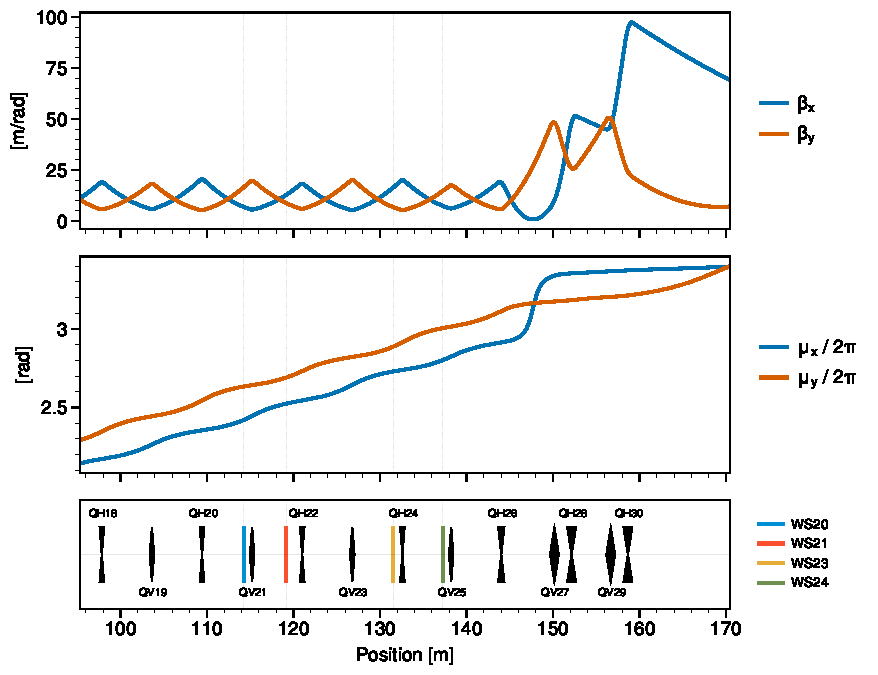
\includegraphics[width=\textwidth]{Images/chapter4/rtbt_optics.pdf}
    \caption{$\beta$ functions, phase advances, and quadrupole/wire-scanner locations in the second half of the RTBT. The plot ends at the spallation target.}
    \label{fig:rtbt_optics}
\end{figure}
%
Each wire-scanner consists of three thin tungsten wires mounted on a fork — one wire is vertical, another is horizontal, and another is tilted at a forty-five-degree angle. The 1D projections of the distribution onto axes perpendicular to the wires are generated by moving the fork across the beam and measuring the charge induced by secondary emission from the wires \cite{Henderson2014}. The four wire-scanners can be run in parallel and take approximately five minutes to move across the beam and return to their original positions. Their step size is 3 mm and their dynamic range is approximately 100. They are run at a beam pulse frequency of 1 Hz.\footnote{Each data point corresponds to a separate beam pulse, so the measurement relies on pulse-to-pulse stability.} The measured profiles can be used to estimate $\langle{xx}\rangle$, $\langle{yy}\rangle$, and $\langle{uu}\rangle$, where the $u$ axis is tilted at angle $\phi = \pi/4$ above the $x$ axis, as well as $\langle{xy}\rangle$ from
%
\begin{equation}
    \langle{xy}\rangle = \frac{\langle{uu}\rangle - \langle{xx}\rangle \cos^2\phi - \langle{yy}\rangle \sin^2\phi}{2\sin\phi\cos\phi}
    .
\end{equation}
%

The SNS employs a target imaging system (TIS) to measure the 2D projection of the distribution on the target \cite{Blokland2010}. The SNS target is a stainless steel vessel containing liquid mercury. Its nose is prepared with a Cr:Al2O3 coating that releases light when impacted by the proton beam. Due to the high-radiation environment, the light is collected by a mirror, deflected, and focused onto an optical fiber bundle which guides the light to a camera some distance away. The TIS configuration is shown in Fig.~\ref{fig:tis}.
%
\begin{figure}[!p]
    \centering
    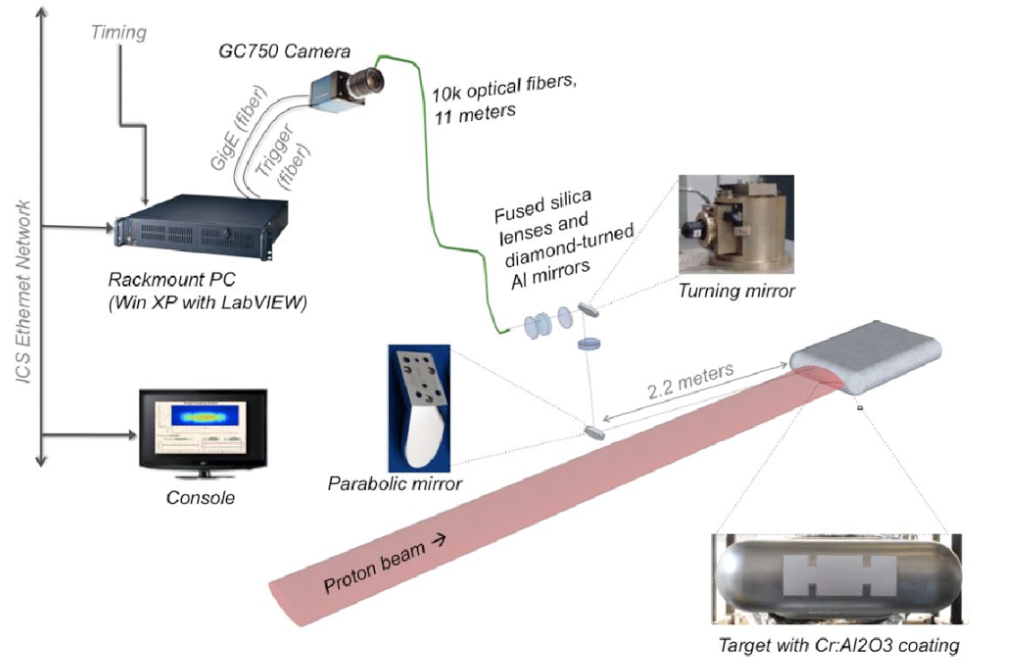
\includegraphics[width=\textwidth]{Images/chapter4/tis1.png}
    \caption{Configuration of the SNS target imaging system. (From \cite{Blokland2010}.)}
    \label{fig:tis}
\end{figure}
%

The optics in the RTBT can be modified, but there are constraints. The $\beta$ functions should be kept below $\approx$ 30 m/rad in the wire-scanner region and below $\approx$ 100 m/rad closer to the target to avoid excess beam loss. At the target, it is best to keep the $\beta$ functions near their default values of $\beta_x \approx$ 60 m/rad and $\beta_y \approx$ 6 m/rad to satisfy peak density and beam size requirements on the target. In addition to these constraints, quadrupoles in the wire-scanner region share power supplies: there is a horizontal group \{QH18, QH20, QH22, QH24\} and a vertical group \{QV19, QV21, QV23, QV25\}. The last five magnets — QH26, QV27, QH28, QV29, and QH30 — are individually controlled.


\section{4D phase space reconstruction from 1D projections}\label{sec:Phase space reconstruction from 1D projections}

\subsection{Method description}

The covariance matrix $\bm{\Sigma}$ can be reconstructed from 1D projections \cite{book:Minty2003, Woodley2000, Prat2014}. We seek to reconstruct $\bm{\Sigma}$ at position $a$ by measuring $\langle{xx}\rangle$, $\langle{yy}\rangle$ and $\langle{xy}\rangle$ at position $b$, downstream of $a$. Assuming linear transport, the two covariance matrices are related by
%
\begin{equation}
    \bm{\Sigma}_b = \mathbf{M} \bm{\Sigma}_a \mathbf{M}^T,
\end{equation}
%
where $\mathbf{M}$ is the linear transfer matrix from $a$ to $b$. We repeat the measurement at least four times with different transfer matrices — either by changing the measurement location or by changing the machine optics — and write
%
\begin{equation}
    \begin{bmatrix}
        {\langle{xx}\rangle}^{(1)} \\
        {\langle{xy}\rangle}^{(1)} \\
        {\langle{yy}\rangle}^{(1)} \\
        {\langle{xx}\rangle}^{(2)} \\
        {\langle{xy}\rangle}^{(2)} \\
        {\langle{yy}\rangle}^{(2)} \\
        {\langle{xx}\rangle}^{(3)} \\
        {\langle{xy}\rangle}^{(3)} \\
        {\langle{yy}\rangle}^{(3)} \\
        \vdots
    \end{bmatrix}_b
    = \mathbf{A}
    \begin{bmatrix}
        \langle{xx}\rangle \\
        \langle{xx'}\rangle \\
        \langle{xy}\rangle \\
        \langle{xy'}\rangle \\
        \langle{x'x'}\rangle \\
        \langle{x'y}\rangle \\
        \langle{x'y'}\rangle \\
        \langle{yy}\rangle \\
        \langle{yy'}\rangle \\
        \langle{y'y'}\rangle \\
    \end{bmatrix}_a
    .
\end{equation}
%
The superscripts represent the measurement index. The transpose of the coefficient matrix $\mathbf{A}$ for a single measurement is
%
\begin{equation}
    \mathbf{A}^T = 
    \begin{bmatrix}
        M_{11}M_{11} & M_{11}M_{31} & M_{31}M_{31} \\
        2M_{11}M_{12} & M_{12}M_{31} + M_{11}M_{32} & 2M_{31}M_{32} \\
        2M_{11}M_{13} & M_{13}M_{31} + M_{11}M_{33} & 2M_{31}M_{33} \\
        2M_{11}M_{14} & M_{14}M_{31} + M_{11}M_{34} & 2M_{31}M_{34} \\
        M_{12}M_{12} & M_{12}M_{32} & M_{32}M_{32} \\
        2M_{12}M_{13} & M_{13}M_{32} + M_{12}M_{33} & 2M_{32}M_{33} \\
        2M_{12}M_{14} & M_{14}M_{32} + M_{12}M_{34} & 2M_{32}M_{34} \\
        M_{13}M_{13} & M_{13}M_{33} & M_{33}M_{33} \\
        2M_{13}M_{14} & M_{14}M_{33} + M_{13}M_{34} & 2M_{33}M_{34} \\
        M_{14}M_{14} & M_{14}M_{34} & M_{34}M_{34}
    \end{bmatrix}
\end{equation}
%
where $M_{ij}$ is the $i$,$j$ element of the transfer matrix for that measurement. The system is solved using linear least squares (LLSQ). 

The measurement has a geometric interpretation, illustrated in Fig.~\ref{fig:ws_emittance_measurement} for the 2D case.
%
\begin{figure}[!p]
    \centering
    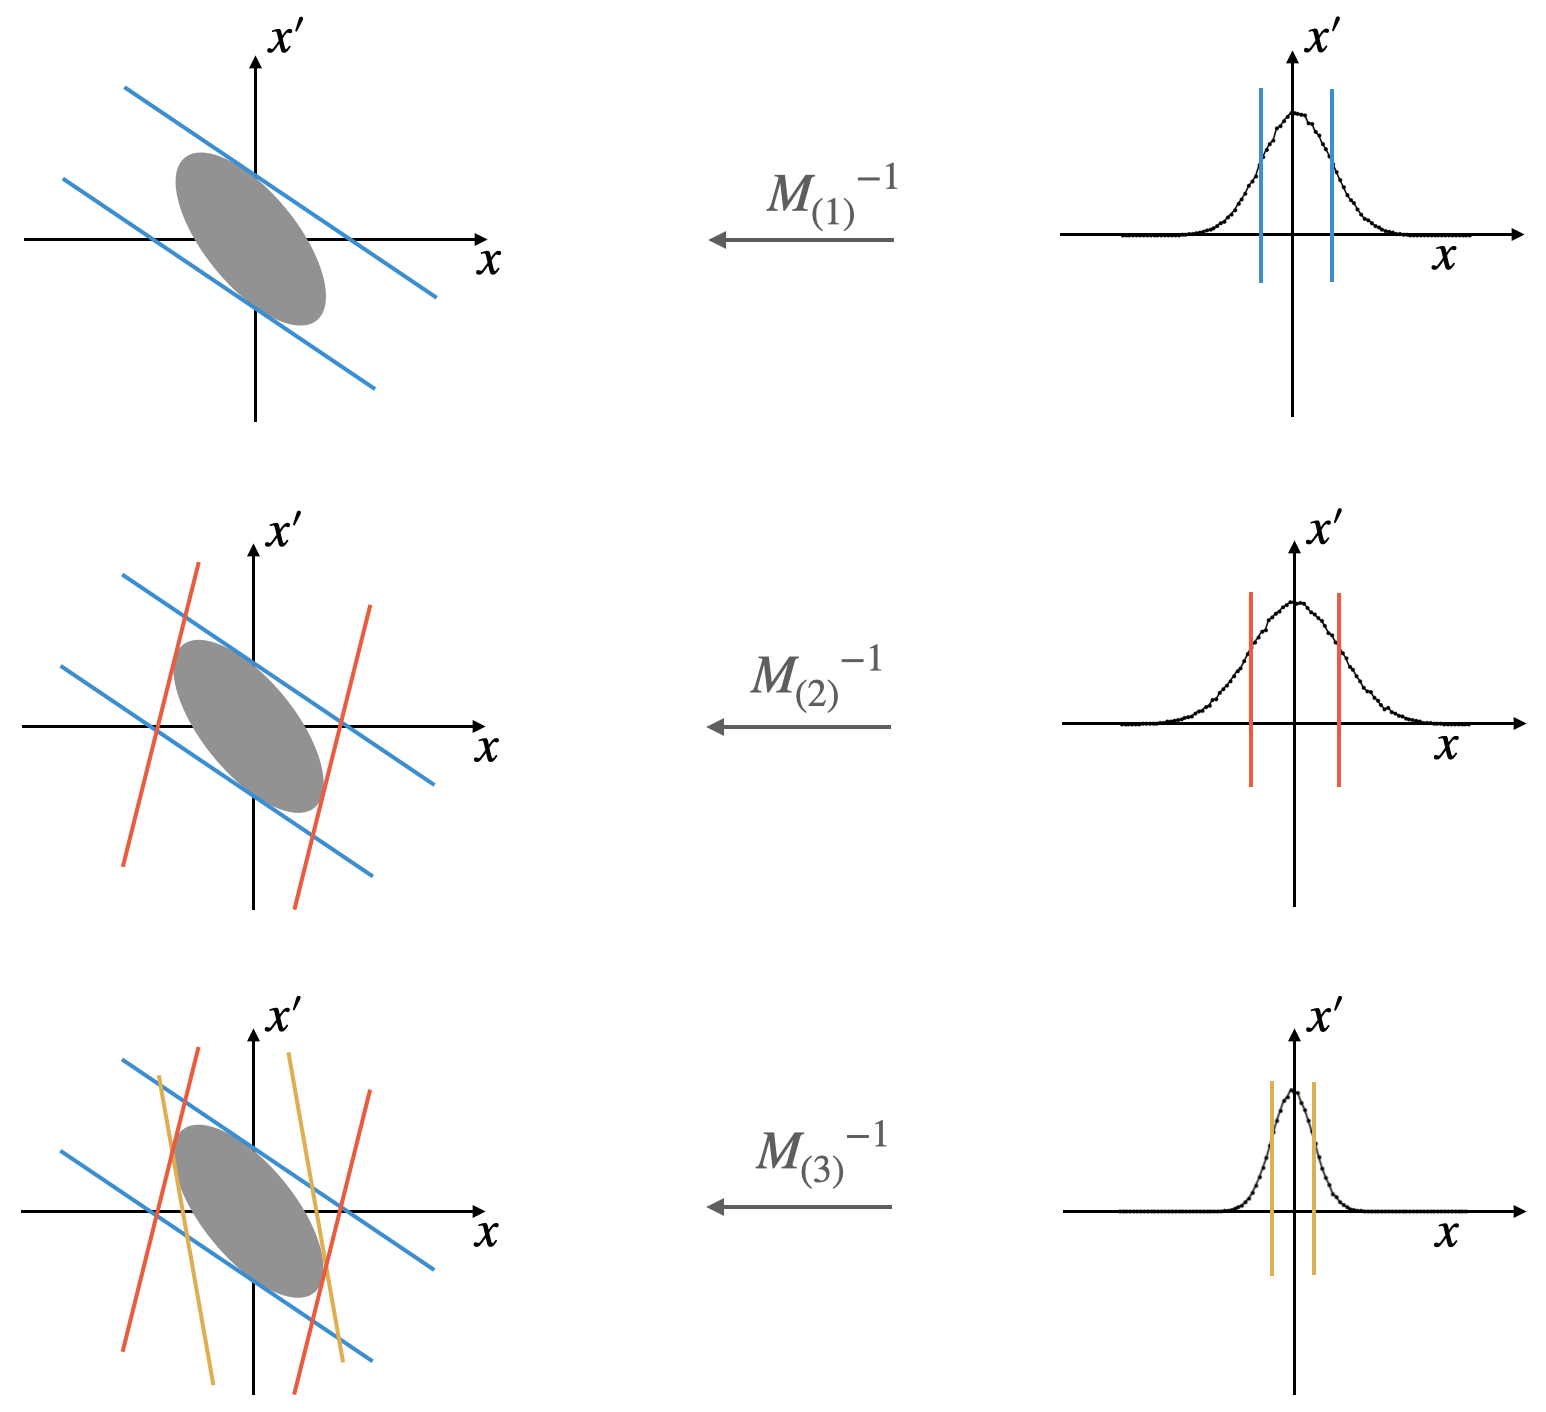
\includegraphics[width=0.9\textwidth]{Images/chapter4/ws_emittance_measurement2.png}
    \caption{Illustration of 2D emittance measurement.}
    \label{fig:ws_emittance_measurement}
\end{figure}
%
Each measured beam size defines two lines in the $x$-$x'$ plane at $b$; when the lines are transported back to $a$, their intersection bounds the phase space ellipse. In the general case, each measurement at $b$ defines a 2D surface in 4D phase space and the intersection of these surfaces at $a$ bounds the phase space ellipsoid.


\subsection{Implementation in the SNS}

To perform the wire scans, the beam is set to a pulse frequency of 1 Hz, and the beam loss monitors in the wire-scanner region are masked due to the higher-than-normal losses when the wires cross the beam core. Wire-scanner data acquisition is performed by the Profile Tools and Analysis (PTA) application. After the four wire-scanners complete their scan, a time-stamped file is produced containing the measured profiles.

The four wire-scanners produce four equations, exactly determining the cross-plane moments, so no optics changes are needed in principle; however, additional measurements should reduce the error. In the 2D case, it is typically recommended to space $n$ measurements by $\pi / n$ in phase advance \cite{book:Minty2003}. This may be due to the geometric interpretation of Fig.~\ref{fig:ws_emittance_measurement}: in normalized phase space, the rotation angle of the measurement lines is equivalent to the phase advance and the lines are evenly spaced around the phase space ellipse. The four wire-scanners in the RTBT are already somewhat evenly spaced in phase advance, and it was determined that a 30$\degree$ window around each wire-scanner would provide sufficient coverage. 

Due to the shared power supplies of the quadrupoles in the wire-scanner region, there is limited control of the phase advances between the wire-scanners. We instead vary the phase advances from QH18 (the first varied quadrupole) to WS24 (the last wire-scanner), which changes the phase advances at WS20, WS21, and WS23 by similar amounts. To set the phase advances at WS24 while constraining the beam size in the wire-scanner region, two power supplies (eight quadrupoles) upstream of WS24 were varied using an optimizer that minimizes the following cost function:
%
\begin{equation}
    C(\mathbf{g}) = \left\Vert{\tilde{\bm{\mu}} - \bm{\mu} }\right\Vert^2
    + 
    \epsilon
    \left\Vert
    \Theta\left(
        \tilde{\bm{\beta}}_{max} - \bm{\beta}_{max}
    \right)
    \right\Vert^2
    .
\end{equation}
%
The quadrupole field strengths are contained in the vector $\mathbf{g}$. The calculated and desired phase advances at WS24 are $\bm{\mu} = (\mu_x, \mu_y)$, and $\tilde{\bm{\mu}} = (\tilde{\mu}_x, \tilde{\mu}_y)$, respectively. The maximum calculated and allowed $\beta$ functions in the wire-scanner region are $\bm{\beta}_{max} = (\beta_{x_{max}}, \beta_{y_{max}})$ and $\tilde{\bm{\beta}}_{max} = (\tilde{\beta}_{x_{max}}, \tilde{\beta}_{y_{max}})$, respectively. $\Theta$ is the Heaviside step function. Finally, $\epsilon$ is a constant.\footnote{We are assuming that the beam is approximately matched to the lattice optics so that the calculated phase advances are close to the true phase advances.}

After the model optics are computed, the live quadrupole settings must be changed. The SNS employs a machine protection system (MPS) that will cause the machine to trip if the RTBT quadrupole strengths wander outside a certain window, so this window is extended beforehand. Additionally, the MPS will activate if the fractional change in field strength is too large; to solve this problem, the field strength is changed in small steps. 

A GUI application to perform the above tasks was developed in the OpenXAL framework for use in the SNS control room. In the first pane of the application, the user can set the phase advances at WS24 and view the model optics and phase advances throughout the RTBT. In the second pane, the user can load wire-scanner output files and choose the reconstruction location. These files contain the wire-scanner profiles, RMS parameters, and Gaussian fit parameters. They also contain an integer that defines the machine state at the time of the measurement. The application reads this number, synchronizes the model with the machine state, and computes the transfer matrices from the wire-scanners to the reconstruction location. The RMS moments and transfer matrices are then used to reconstruct the covariance matrix. The resulting beam parameters are printed and compared to the model lattice parameters. The 2D projections of the covariance ellipsoid are plotted along with the measurement lines, with the option to view in normalized coordinates. 



\subsection{Measurement of a production beam}

The multi-optics method was tested on a fully accumulated production beam. The phase advances at WS24 were varied in a 30$\degree$ range over ten steps: the first half of the scan held the vertical phase advance fixed while varying the horizontal phase advance, and the second half of the scan held the horizontal phase advance fixed while varying the vertical phase advance. The result of the reconstruction is shown in Fig.~\ref{fig:prod_meas} for a location just before QH18.
%
\begin{figure}[!p]
    \centering
    \begin{subfigure}{0.9\textwidth}
        \centering
        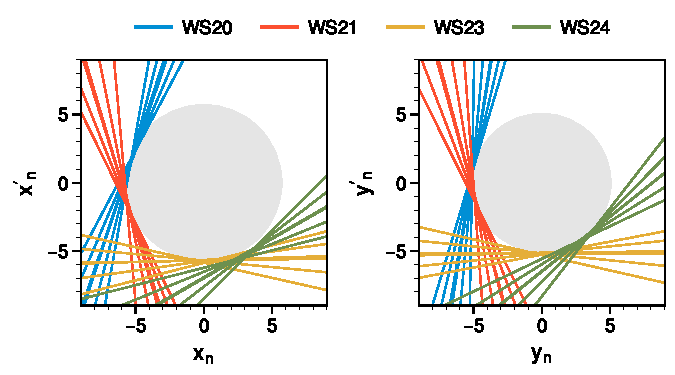
\includegraphics[width=\textwidth]{Images/chapter4/prod_meas_lines.pdf}  
    \end{subfigure}
    \par\medskip
    \begin{subfigure}{0.6\textwidth}
        \centering
        \begin{tabular}{lll}
            \small\textbf{Parameter} & \small\textbf{Measurement} & \small\textbf{Model} \\
            \midrule
            \small$\beta_x$ [m/rad] & \small22.06 $\pm$ 0.29 & \small22.00 \\
            \small$\beta_y$ [m/rad] & \small4.01 $\pm$ 0.02 & \small3.81 \\
            \small$\alpha_x$ & \small2.33 $\pm$ 0.04 & \small2.37 \\
            \small$\alpha_y$ & \small-0.49 $\pm$ 0.01 & \small-0.60 \\
            \small$\varepsilon_1$ [mm~mrad] & \small33.02 $\pm$ \small0.05 & - \\
            \small$\varepsilon_2$ [mm~mrad] & \small25.67 $\pm$ \small1.03 & - \\
            \small$\varepsilon_x$ [mm~mrad] & \small32.85 $\pm$ \small0.05 & - \\
            \small$\varepsilon_y$ [mm~mrad] & \small25.87 $\pm$ \small0.12 & - \\
          \end{tabular}
    \end{subfigure}
    \par\medskip
    \caption{Reconstructed beam parameters and graphical output from a multi-optics emittance measurement of a production beam.}
    \label{fig:prod_meas}
\end{figure}
%
The best-fit ellipses in the $x$-$x'$ and $y$-$y'$ planes are normalized by the reconstructed Twiss parameters. The uncertainties in the beam parameters were calculated by propagating the standard deviations of the ten reconstructed moments obtained from the LLSQ estimator.\footnote{See Appendix A of \cite{Faus-Golfe2016}.} The reconstructed Twiss parameters are close to the model parameters computed from the linear transfer matrices of the ring and RTBT, showing that the beam is matched. The intrinsic emittances are almost equal to the apparent emittances, showing that there is very little cross-plane correlation in the beam. This is expected for a production beam.



\subsection{Sensitivity to errors}

A comprehensive study of errors in the multi-optics 4D emittance measurement was completed at the SwissFEL Injector Test Facility (SITF) by Prat and Aiba in \cite{Prat2014}. They considered errors in the measured moments, quadrupole field and alignment errors, beam energy errors, beam mismatch at the reconstruction point, and dispersion/chromaticity \cite{Mostacci2012}, concluding that the multi-optics measurement remained accurate, reporting $< 5\%$ uncertainty in the intrinsic emittances. We initially performed similar studies in PyORBIT using envelope tracking to estimate the reconstruction errors in the RTBT, also concluding that the method should remain accurate \cite{Hoover2021-IPAC}. Space charge forces, which can render the method invalid for high-perveance beams \cite{Anderson2002}, can be neglected: the space charge tune shift in the ring is around 3\%, and the distance between the reconstruction and measurement locations is much smaller than the length of the ring. 

In summary, the multi-optics emittance measurement is feasible in the SNS. The only downside is the long measurement time, for the following reasons. First, we are not only interested in the beam emittances at a single time but are also interested in the growth and evolution of the emittances throughout accumulation. For example, it could be possible for $\varepsilon_2$ to remain small (as desired) in the first half of accumulation before growing to a much larger value in the second half of accumulation. Measurement of this emittance evolution would convey valuable information about the beam dynamics and allow for qualitative comparison with computer simulation. Second, it would be beneficial to quickly evaluate various machine states, the best of which will be unknown during initial experiments. Finally, a practical point: the time reserved for accelerator physics (AP) experiments at the SNS is limited, and the setup for initial experiments will be much longer than typical AP experiments for reasons not discussed in this paper. Thus, the fixed-optics method is preferred, in which only four profiles are used in the reconstruction. A modest reduction in accuracy for the increase in speed is warranted since weak cross-plane correlations ($\varepsilon_1 \varepsilon_2 \approx \varepsilon_x \varepsilon_y$) are uninteresting for our purposes and do not need to be resolved. 

Using only one set of optics from the previous scan resulted in a covariance matrix that was not positive-definite, producing imaginary intrinsic emittances. We label this a failed fit. A nonlinear solver \cite{Raimondi1993} or Cholesky decomposition \cite{Agapov2007} can be used to ensure a valid covariance matrix, but we found that the answer depended strongly on the initial guess provided to the solver and on which measurement in the scan was used in the reconstruction.

To investigate the failure of the fixed-optics method, a covariance matrix was generated with cross-plane moments set to zero and within-plane moments matched to the lattice optics, then tracked to the wire-scanners using the known transfer matrices. The reconstruction was then performed 1000 times with 3\% random noise added to the moments.\footnote{To select the proper noise level, the wire-scanners were run seven times without changing the machine optics, producing seven estimated moments for each of the three wires on each of the four wire-scanners. The profiles are highly reproducible: for each wire, the maximum difference between any two moments was always less than 3\% of the mean moment. Therefore, the noisy moments were sampled within $\pm$ 3\% of the true moments.} Failed fits were discarded. Fig.~\ref{fig:prod_sensitivity} shows that the reconstructed intrinsic emittances in the successful trials are very sensitive to changes to the ``measured" moments. 
%
\begin{figure}[!p]
    \vspace*{5cm}
    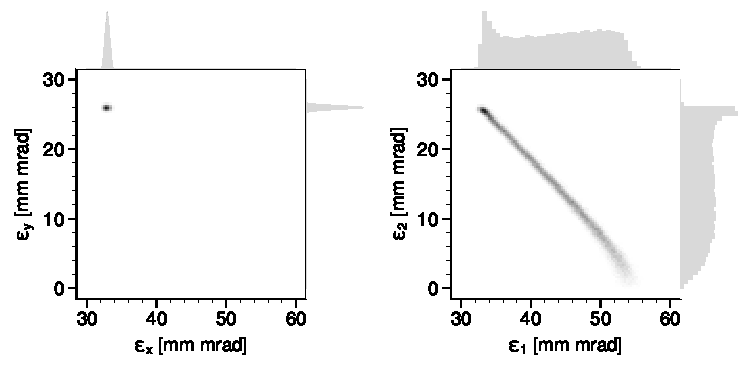
\includegraphics[width=\textwidth]{Images/chapter4/prod_sensitivity.pdf}
    \caption{Monte Carlo simulation of a fixed-optics emittance measurement in the RTBT. Trials were repeated until several thousand successful fits were obtained. 3\% noise was assumed for the measured moments. Transfer matrix errors were ignored. The correct values are $\varepsilon_1$ = $\varepsilon_x$ = 32 mm~mrad, $\varepsilon_2$ = $\varepsilon_y$ = 20 mm~mrad.}
    \label{fig:prod_sensitivity}
    \vspace*{5cm}
\end{figure}
%
Unlike the apparent emittances, the intrinsic emittances are strongly correlated and are not centered on the correct values. We refer to the difference between the mean emittances and the true emittances as the \textit{bias}. The reason for the bias is that $\varepsilon_1\varepsilon_2 \le \varepsilon_x\varepsilon_y$.

Sensitivity of fixed-optics 4D emittance measurements was observed by Woodley and Emma \cite{Woodley2000} and studied more recently by Agapov, Blair, and Woodley \cite{Agapov2007} as well as Faus-Golfe et al. \cite{Faus-Golfe2016}, all in the context of design studies for a future International Linear Collider (ILC). The motivation for these studies is that a flat beam ($\varepsilon_y \ll \varepsilon_x$) would be ideal for the ILC, and that $\varepsilon_y$ can be minimized by measuring and removing any cross-plane correlation in the beam. Woodley and Emma proposed to abandon the fixed-optics method due to the bias in the reconstructed intrinsic emittances introduced by large errors in the measured moments, suggesting to instead measure the 2D emittance and iteratively minimize $\varepsilon_y$. 

Agapov, Blair, and Woodley revisited this problem and showed that the linear system used to reconstruct the cross-plane moments can easily become ill-conditioned. The sensitivity of a linear system $\mathbf{A} \mathbf{x} = \mathbf{b}$ to errors in $\mathbf{b}$ is determined by the condition number $C = \Vert \mathbf{A} \Vert \Vert \mathbf{A}^{-1} \Vert$ (or the pseudo-inverse $\mathbf{A}^\dagger = (\mathbf{A}^T\mathbf{A})^{-1} \mathbf{A}^T$ if $\mathbf{A}$ is not square) where $\Vert \dots \Vert$ is a matrix norm \cite{Golub1985}. As an example, consider four wire-scanners that are evenly spaced in phase advance and connected by rotation matrices. Since the transfer matrices are uncoupled, there are three independent subsystems to solve: $x$-$x'$, $y$-$y'$, and the cross-plane moments. Let the coefficient matrices for these subsystems be $\mathbf{A}_{xx}$, $\mathbf{A}_{yy}$, and $\mathbf{A}_{xy}$, respectively, and the condition numbers be $C_{xx}$, $C_{yy}$, and $C_{xy}$. Recall that the within-plane moments are overdetermined while the cross-plane moments are exactly determined. Fig.~\ref{fig:fodo_condition_number} plots the inverse of these condition numbers as a function of the wire-scanner spacing.
%
\begin{figure}[!p]
    \centering
    \vspace*{2cm}
    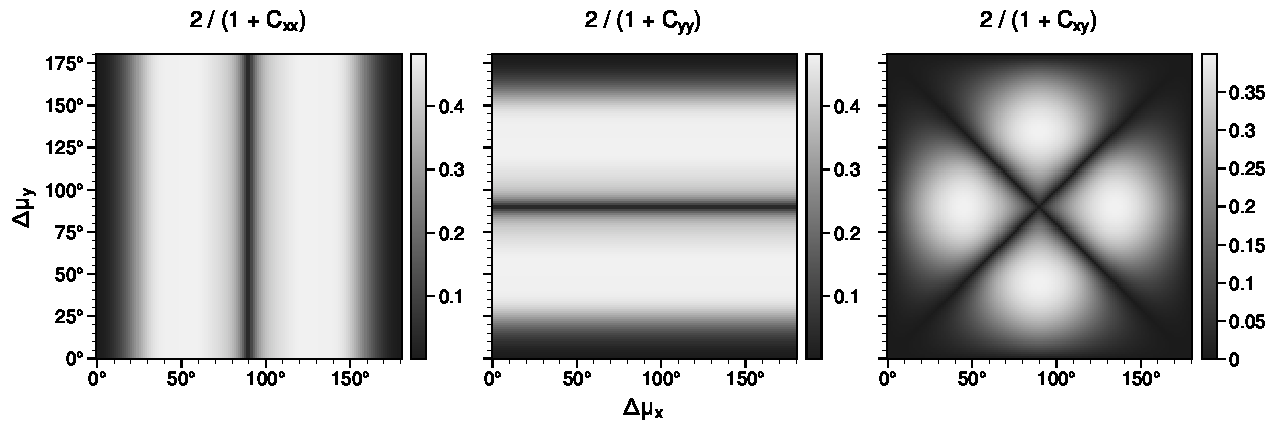
\includegraphics[width=\textwidth]{Images/chapter4/fodo_condition_number.pdf}
    \caption{Condition numbers of the coefficient matrices for four wire-scanners that are evenly spaced in phase advance and connected by rotation matrices.}
    \label{fig:fodo_condition_number}
    \vspace*{2cm}
\end{figure}
%
$C_{xx}$ and $C_{yy}$ approach $\infty$ when the spacing is $\pi/2$ in their respective planes, in which case two pairs of measurements provide degenerate information, while $C_{xy}$ depends on the difference between the phase advances. The pattern will be more complicated for different optics and/or additional wire-scanners. The error and uncertainty in the emittance reconstruction, as well as the number of failed fits, mirrors these condition numbers. Using this framework, Faus-Golfe et al. developed analytical formulas to determine whether a given system can accurately measure the intrinsic emittances. They also suggested that the planned ILC emittance measurement station, which contained four wire-scanners, could be modified to reduce the sensitivity. 

We performed a similar modification to the RTBT wire-scanner region. To find a new set of optics, the phase advances at WS24 ($\mu_x$, $\mu_y$) were varied in a $90\degree$ window centered on their nominal values ($\mu_{x0}$, $\mu_{y0}$); at each setting, the condition numbers were calculated and the reconstruction was simulated with true emittances $\varepsilon_x  = \varepsilon_y = \varepsilon_1 = \varepsilon_2$ = 20 mm~mrad. Failed trials were discarded. The resulting biases and standard deviations of the reconstructed emittances are plotted in Fig.~\ref{fig:rtbt_montecarlo_emittances}.
%
\begin{figure}[!p]
    \centering
    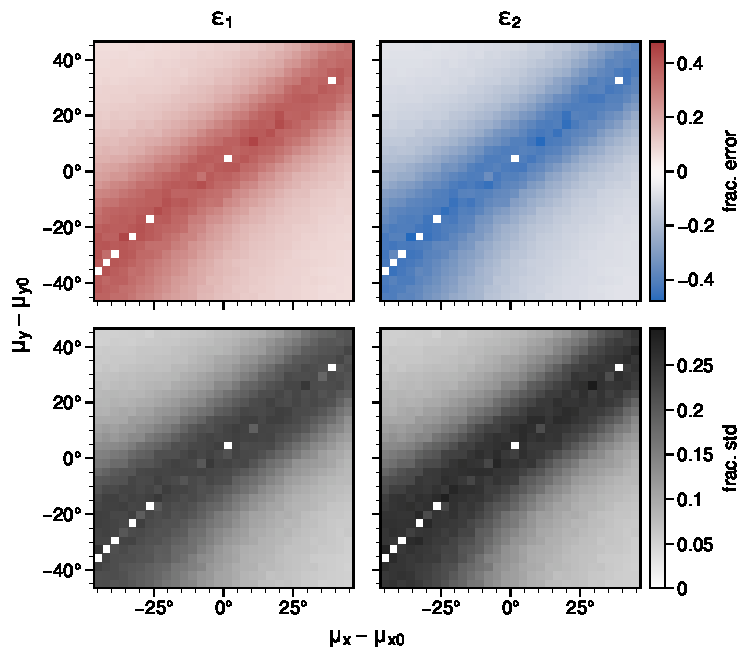
\includegraphics[width=0.9\textwidth]{Images/chapter4/rtbt_montecarlo_emittances.pdf}
    \caption{Simulated 4D emittance reconstruction errors as a function of the phase advances at WS24.}
    \label{fig:rtbt_montecarlo_emittances}
\end{figure}
%
Settings that produced no successful trials appear as white cells. The apparent emittances are not displayed because they remained within 1\% of their true values at every optics setting. Modifying the optics so that $\mu_x = \mu_{x0} + 45\degree$, $\mu_y = \mu_{y0} - 45\degree$ reduces the bias to $\approx 7\%$ and the standard deviation to $\approx 5\%$. The fraction of failed fits, which is very large along the diagonal in the figure, is reduced to zero.

It is also important to examine the effect of mismatched beam parameters on the accuracy of the reconstruction. Recall that the phase advance is the integral of the inverse of the $\beta$ function. In a periodic system, there is a unique periodic solution for the $\beta$ function, but this is not true in a transfer line such as the RTBT; thus, the phase advance in the RTBT depends on the Twiss parameters at the ring extraction point — the RTBT entrance. 

All previous phase advance calculations have assumed that the beam Twiss parameters are the same as the ring Twiss parameters at extraction. This is generally a safe assumption since turn-by-turn mismatch oscillations are washed out during painting. It is possible, however, for space charge to effectively modify the ring Twiss parameters, resulting in mismatch when entering the RTBT. This modification is small during production painting, as shown in Fig.~\ref{fig:prod_meas}, but it is expected (from simulations) that more significant mismatch could occur if the space charge density is increased and/or if the beam energy is decreased.

To examine the effect of mismatch, we first moved the operating point to $\mu_x = \mu_{x0} + 45\degree$, $\mu_y = \mu_{y0} - 45\degree$, then varied the initial Twiss parameters at BPM17 in the RTBT and repeated the Monte Carlo trials. There are four parameters: $\alpha_x$, $\alpha_y$, $\beta_x$, and $\beta_y$. We based the range of each parameter on a measurement in which the reconstructed Twiss parameters were different than the nominal Twiss parameters, shown in Table~\ref{tab:mismatch}.  
%
\begin{table}[!p]
    \centering
    \caption{Reconstructed and model Twiss parameters at BPM 17 in the RTBT (see Experiment 2 in Chapter \ref{chap-5}.)}
    \begin{tabular}{lll}
    \midrule
    \textbf{Parameter} & \textbf{Measured} & \textbf{Model} \\
    \midrule
    $\beta_x$ [m/rad] & 6.26 & 5.49 \\
    $\beta_y$ [m/rad] & 20.82 & 19.25 \\
    $\alpha_x$ & -0.89 & -0.78 \\
    $\alpha_y$ & 1.17 & 1.91 \\
    \midrule    
    \end{tabular}
    \label{tab:mismatch}
\end{table}
%
The beam mismatch is unlikely to exceed these values in future experiments.\footnote{Details about the measurement are left for Chapter \ref{chap-5}.} Therefore, to examine the effect of mismatch, we first moved the operating point to $\mu_x = \mu_{x0} + 45\degree$, $\mu_y = \mu_{y0} - 45\degree$, then varied $\beta_x$ and $\beta_y$ within a $\pm 20\%$ window around their model values, $\alpha_x$ within a $\pm 15\%$ window, and $\alpha_y$ within a $-40\%, +10\%$ window to extend beyond the measured discrepancies, and repeated the Monte Carlo trials for each initial beam, thus producing a collection of means and standard deviations for the reconstructed intrinsic emittances. The left plot in Fig.~\ref{fig:mismatch} displays the standard deviations and biases for $\varepsilon_1$ (pink) and $\varepsilon_2$ (blue).
%
\begin{figure}[!p]
    \centering
    \includegraphics[width=\textwidth]{Images/chapter4/mismatch2.pdf}
    \caption{Bias and standard deviation of $\varepsilon_1$ (pink) and $\varepsilon_2$ (blue) from simulated reconstructions in the RTBT. In each plot, the collection of points is generated by varying the initial beam Twiss parameters. The true values of the emittances are printed on the top of the figures.}
    \label{fig:mismatch}
\end{figure}
%
Although most of the points are clustered near the original bias and standard deviation of 7\% and 5\%, respectively, the bias increases to nearly 15\% in some cases, which may make it difficult to resolve weak cross-plane correlation; however, the measurement should still resolve strong cross-plane correlation. This is demonstrated in the rest of the plots in Fig.~\ref{fig:mismatch}, in which the entire process is repeated with $\varepsilon_1 / \varepsilon_2 > 1$. The bias in the reconstruction quickly decreases — the emittances are clustered around their true values. 

We conclude that with small modifications to the RTBT optics, the fixed-optics method should be sufficient for fast 4D emittance measurements in the SNS. As detailed in Chapter 5, such measurements will be needed to evaluate various machine settings within a single study period, especially in initial experiments, as well as to measure the emittance growth during accumulation for qualitative comparison with simulation. The multi-optics method should be used once a promising machine state is found (or if time allows) to reduce the uncertainty.


\subsubsection{Other uses of 1D projections}

To close this section, we mention that there is information to be gained from 1D projections in addition to the root-mean-square reconstruction just described. First, the measured projections can be compared to the ideal ``half-circle" projections of a uniform density ellipse.\footnote{The best expected case is a uniform density core with small nonlinear tails, the 1D projection of which is distinguishable from a Gaussian curve, but it may be difficult to distinguish intermediate cases with larger tails. The method we employ in the next chapter is to calculate the standard deviation of the measured profile, plot the projections of an ideal Gaussian and uniform density elliptical distribution with the same standard deviation, and visually compare the three curves. More quantitative methods may be used in the future.} Second, the projections can be used to reconstruct the $x$-$x'$ or $y$-$y'$ distribution using the tomographic methods described in the next section; it may be possible to include cross-plane information in the reconstruction using diagonal projections. 


\section{4D phase space reconstruction from 2D projections}

Tomographic methods are well-established for the reconstruction of 2D phase space distributions from 1D projections in transverse phase space \cite{Hock2014} and longitudinal phase space \cite{Evans2014}. The concept has recently been extended to the reconstruction of the 4D transverse phase space, both in theory and in practice \cite{Hock2013b, Wang2019, Wolski2020}. This section begins with a brief discussion of tomography in two dimensions as applied to beam diagnostics, then moves on to describe the accuracy and limitations of several 4D reconstruction algorithms. Finally, the use of tomography to reconstruct the 4D phase space distribution from beam images on the SNS target is discussed. 



\subsection{Tomography for beam diagnostics}

Several algorithms exist to reconstruct 2D images from 1D projections, such as filtered back-projection (FBP), algebraic reconstruction (ART) \cite{Slaney1988}, and maximum entropy (MENT) \cite{Minerbo1979}. Projections of an object are normally obtained by illuminating the object at different angles. Although the measured projections of a 2D phase space distribution ($x$-$x'$) are always along the $x$ axis, we can take advantage of the known transfer matrix $\mathbf{M}$ between the measurement location $b$ and the reconstruction location $a$ to obtain the projections at different angles in $x$-$x'$ at the reconstruction location. The measured projection of the $x$-$x'$ distribution at $b$ is
%
\begin{equation}
    p_b(x_b) = \int_{-\infty}^{\infty} f(x_b, x'_b) dx'_b.
\end{equation}
%
When the distribution is transported back to $a$, the projection will be along axis $\tilde{x}_a$, which is rotated at angle $\theta$ above the $x_a$ axis. The projection angle is computed from the transfer matrix \cite{Hock2013a}:
%
\begin{equation}\label{eq:proj_trans_1}
    \tan\theta = \frac{M_{12}}{M_{11}}.
\end{equation}
%
The distance along the projection axis will be scaled:
%
\begin{equation}\label{eq:proj_trans_2}
    r = \frac{x_b}{\tilde{x}_a} = \sqrt{M_{11}^2 + M_{12}^2}.
\end{equation}
%
The projection must then be scaled to conserve its area. The projections at $a$ and $b$ are related by 
%
\begin{equation}\label{eq:proj_trans_3}
    p_a(\tilde{x}_a) = r p_b(r \tilde{x}_a).
\end{equation}
%
Standard tomography algorithms can be applied to the scaled projections.

Reconstructing the distribution in normalized phase space can reduce errors \cite{Hock2011}. Recall the normalization matrix $\mathbf{V}$ from Eq.~\eqref{eq:CS_parameterization}. Note that
%
\begin{equation}
\begin{aligned}
    \mathbf{x}_b 
    = \mathbf{M} \mathbf{x}_a
    = \mathbf{M} \mathbf{V} (\mathbf{V}^{-1} \mathbf{x}_a)
    ,
\end{aligned}
\end{equation}
%
where $\mathbf{V}$ depends on the Twiss parameters at $a$. Eq.~\eqref{eq:proj_trans_1}, Eq.~\eqref{eq:proj_trans_2}, and Eq.~\eqref{eq:proj_trans_3} can be applied to the matrix $\mathbf{M} \mathbf{V}$ to obtain the projections in the normalized phase space at $a$. After the image is reconstructed, the true distribution can be obtained by transforming the grid coordinates using $\mathbf{V}$ and interpolating at the transformed coordinates. Any Twiss parameters can be used to form $\mathbf{V}$; if the Twiss parameters are matched to the distribution, the rotation angle of the projection will be the phase advance from $a$ to $b$, and the reconstructed distribution will be circular in the normalized phase space. 


\subsection{4D reconstruction as a series of 2D reconstructions}

Recent work by Hock et al. reduces 4D reconstruction to a series of 2D reconstructions when the $x$-$y$ projections are available \cite{Hock2013a}. The method, which we refer to as Hock's method, is as follows. Assume that the rotation angles in $x$-$x'$ and $y$-$y'$ can be independently controlled. Let the angles in $x$-$x'$ be \{$\theta_{x_1}$, $\dots$, $\theta_{x_k}$, $\dots, \theta_{x_K}$\} and the angles in $y$-$y'$ be \{$\theta_{y_1}$, $\dots$, $\theta_{y_l}$, $\dots$, $\theta_{y_L}$\}. The projections are stored in an array $\mathbf{S}$, where $\mathbf{S}_{i,j,k,l}$ is the intensity at point ($x_i$, $y_j$) on the screen for angles $\theta_{x_k}$, $\theta_{y_l}$. Consider a single row of an image, fixing $y_j$, which gives a 1D projection of a slice of the distribution onto the $x$-axis at the screen. If we fix $\theta_{y}$ and vary $\theta_{x}$, we produce a set of 1D projections that can be used to reconstruct the $x$-$x'$ phase space distribution for this slice using any 1D $\rightarrow$ 2D reconstruction method. This is repeated for each $y_j$ and $\theta_{y_l}$. Now, for each $x$ and $x'$ in the reconstruction grid, we have set of projections of the $y$-$y'$ distribution onto the $y$-axis at the screen for different $\theta_{y}$; thus, for each $x$ and $x'$ in the reconstruction grid, we can reconstruct the $y$-$y'$ distribution. This completes the reconstruction.

To test the method, the 600,000-particle distribution from Fig.~\ref{fig:Holmes} was used. In \cite{Hock2013a}, filtered back-projection (FBP) was used for the 2D reconstructions. FBP requires many projections — something that is not always possible in the context of beam diagnostics. Simultaneous algebraic reconstruction (SART) is a possible alternative when the number of projections is small. The accuracy of SART will depend on the number of projections and the range of projection angles. Fig.~\ref{fig:tomo_sim_art2D} demonstrates this by reconstructing the $y$-$y'$ distribution from 1D projections as these numbers are varied.
%
\begin{figure}[!p]
    \centering
    \vspace*{3.0cm}
    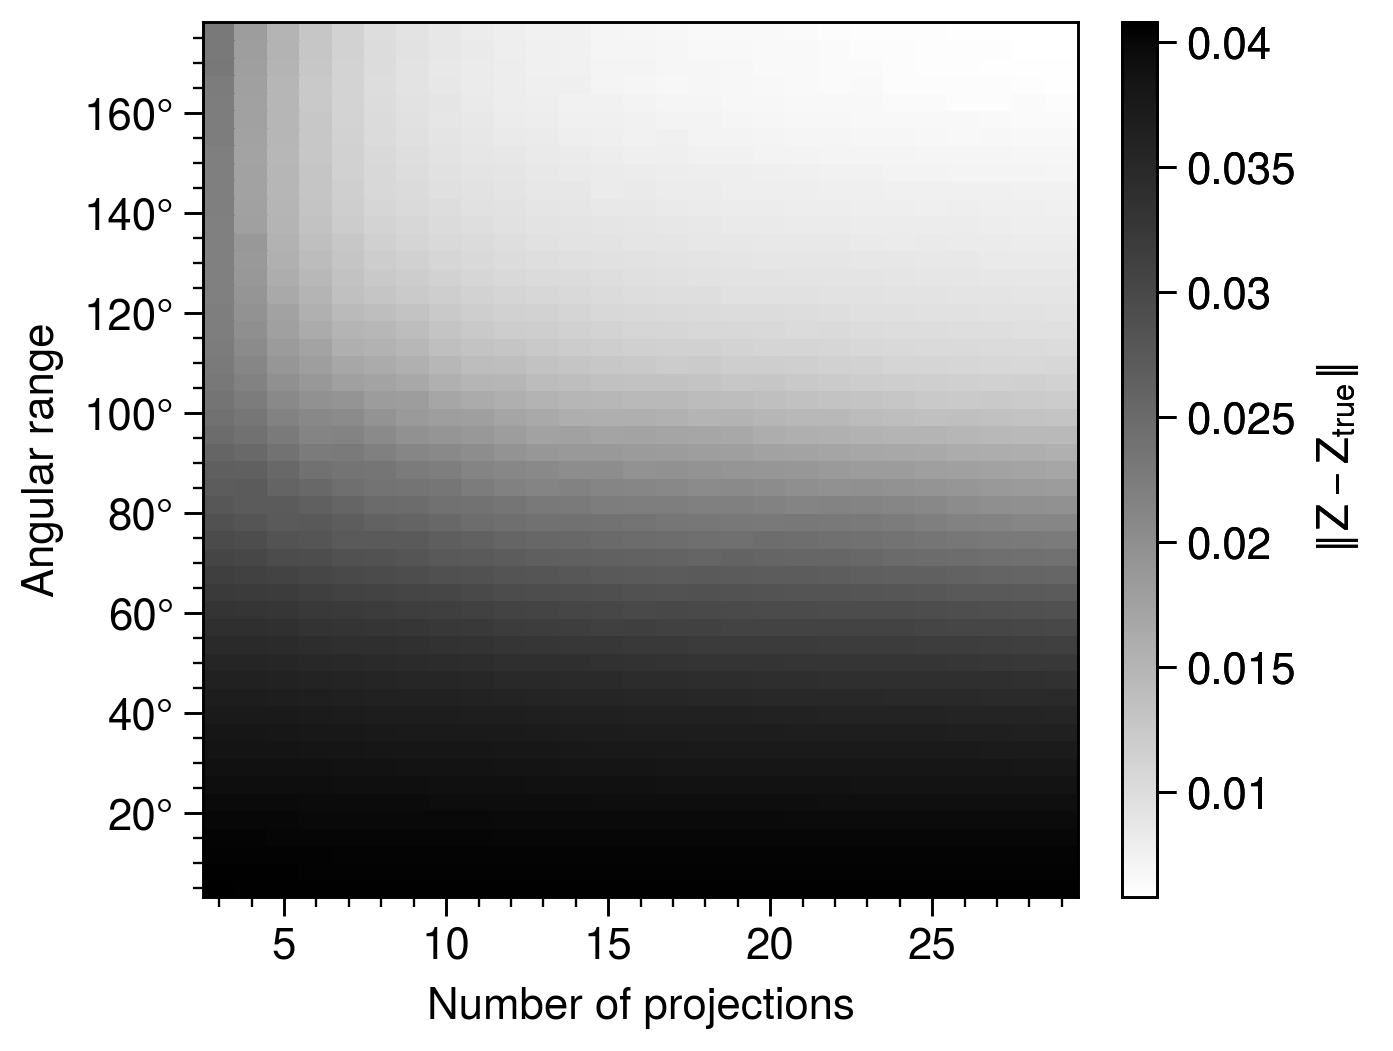
\includegraphics[width=0.6\textwidth]{Images/chapter4/tomo_sim_art2d.png}
    \caption{Test of SART accuracy as a function of number of projections and range of projection angles.}
    \label{fig:tomo_sim_art2D}
    \vspace*{3.0cm}
\end{figure}
%
It appears that if the projection angles are distributed over a significant range, the accuracy does not improve much beyond 10-15 projections. As discussed later, 15 projections are likely near the maximum possible in the SNS for each 2D reconstruction if using Hock's method. In the following simulated 4D reconstruction, the phase advances in both planes were scanned over $180\degree$ in 12 steps; at each step, the distribution was transported to and then binned on a virtual screen. The reconstruction was performed in normalized phase space, and it was assumed that the distribution was matched to the lattice parameters. Fig.~\ref{fig:tomo_sim_target_scan} shows the simulated images in normalized space with a screen resolution of $75 \times 75$.
%
\begin{figure}[!p]
    \centering
    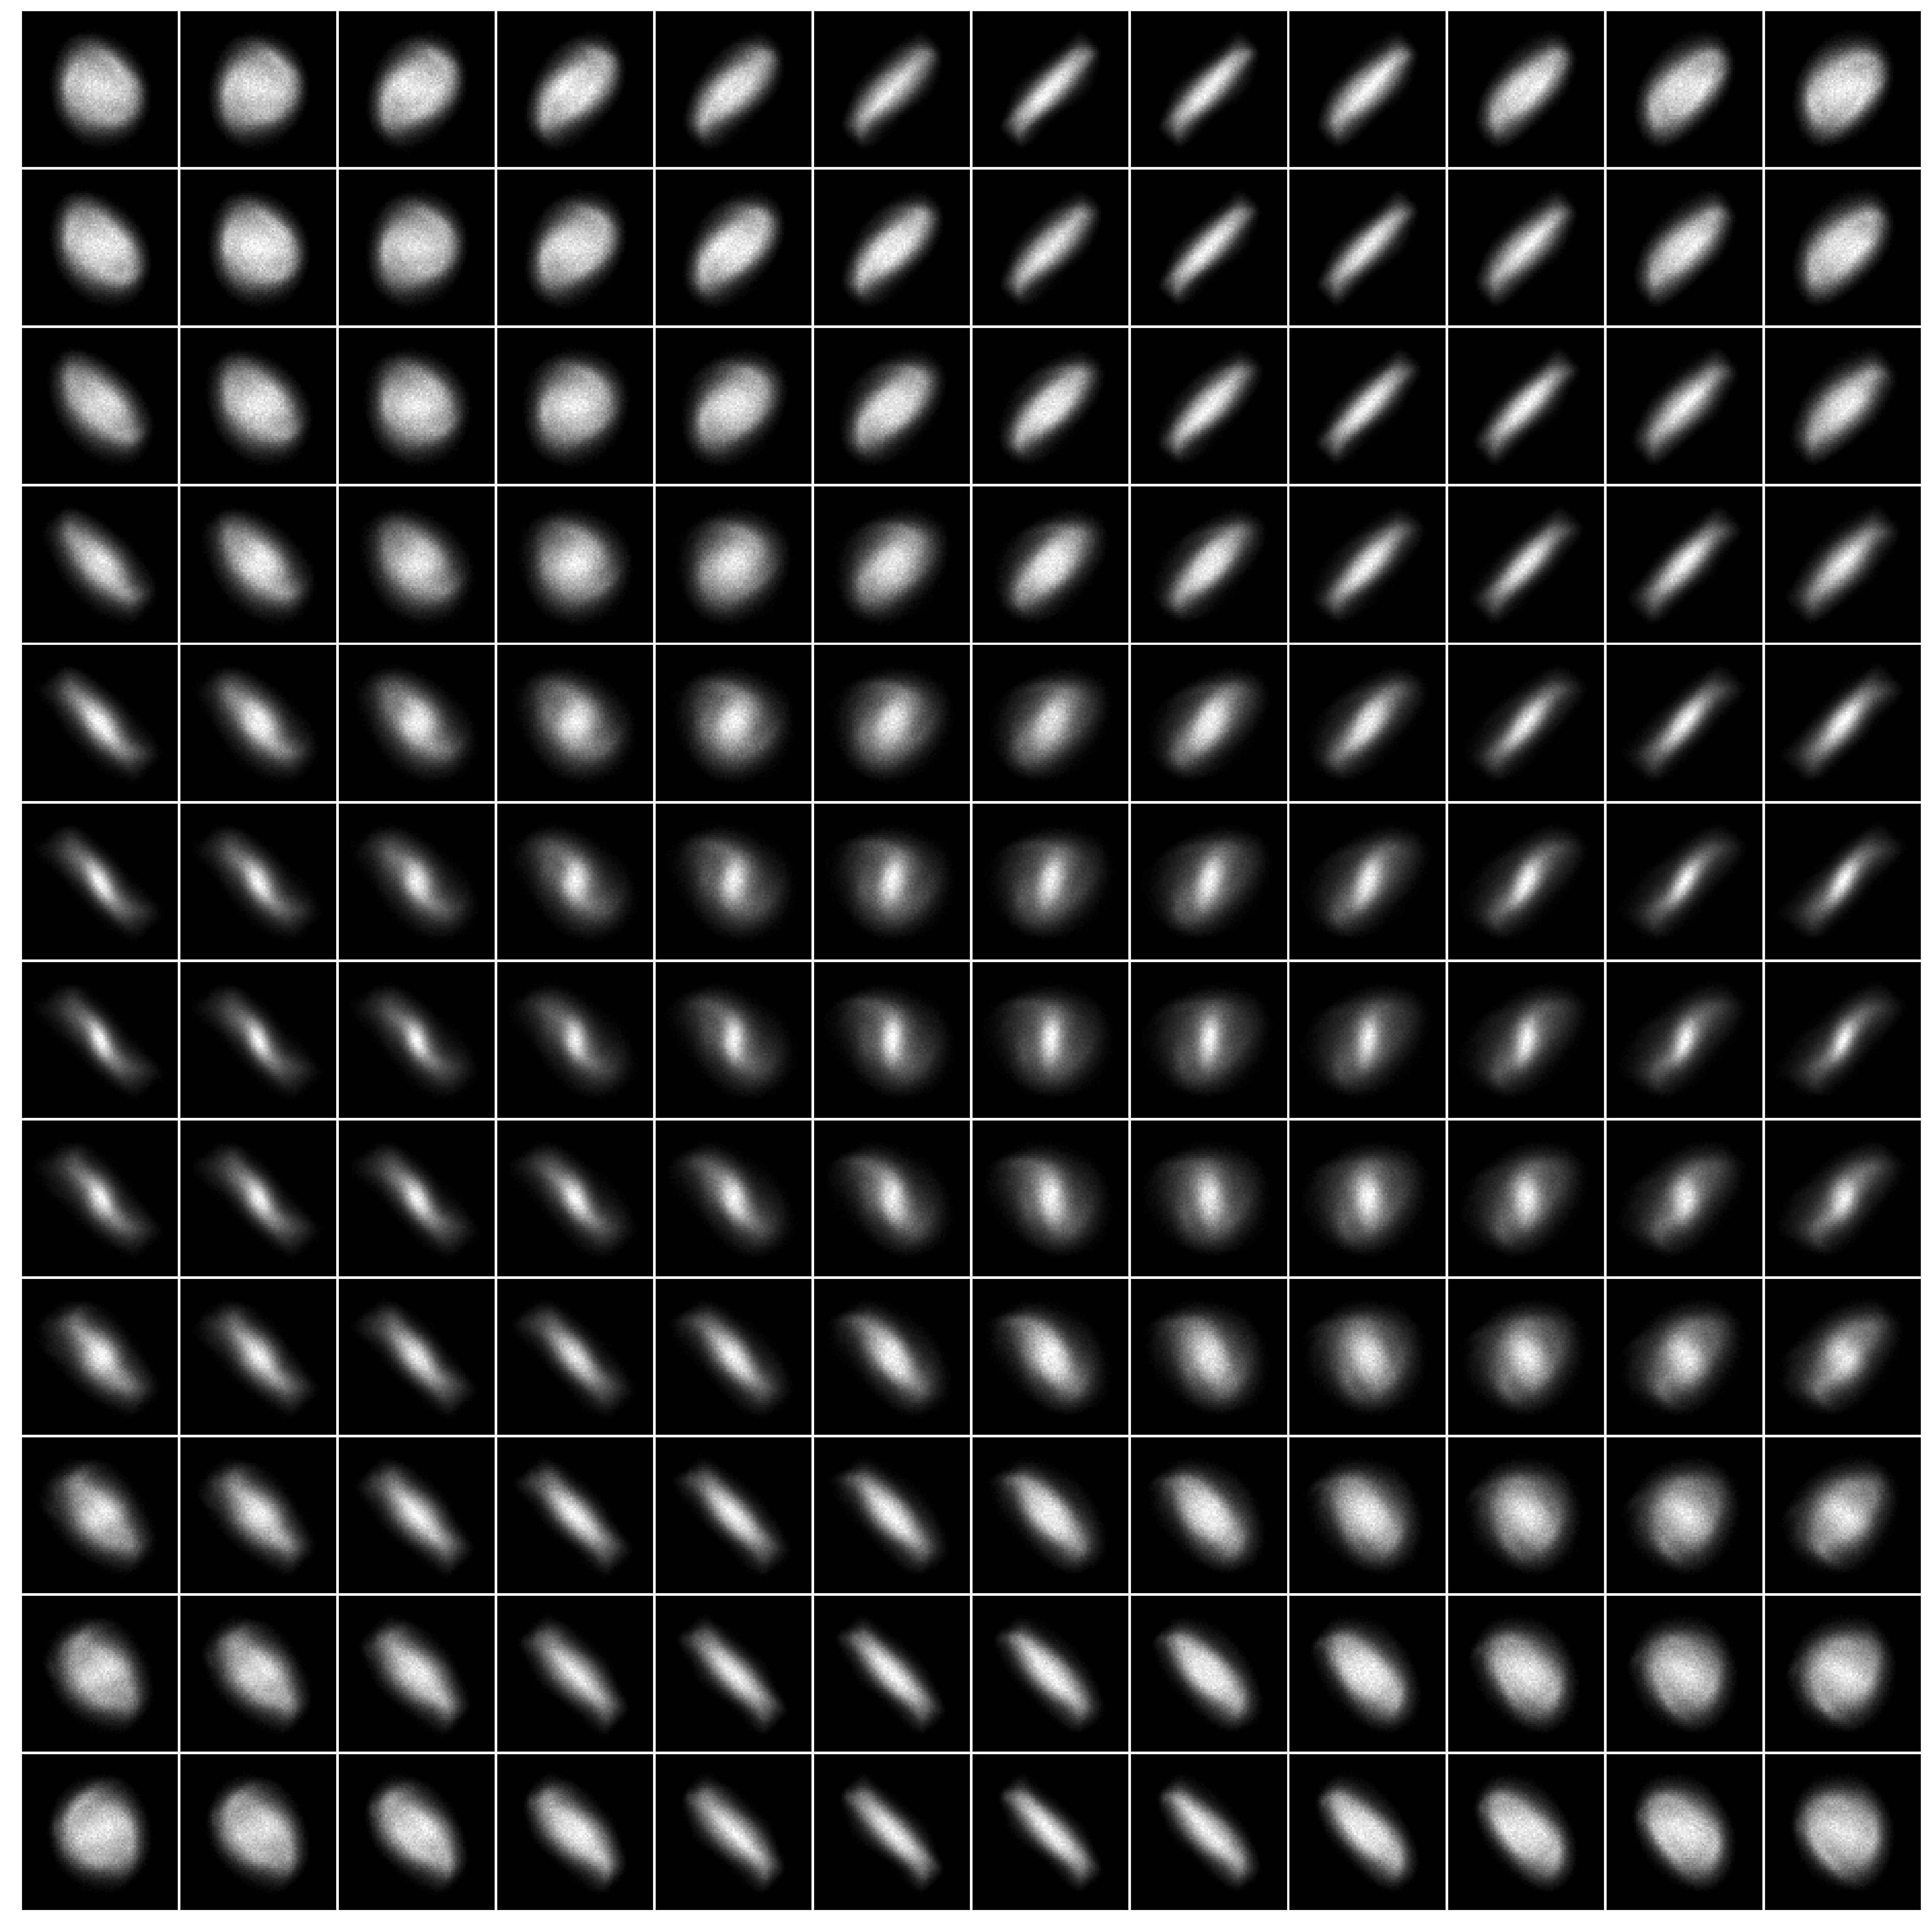
\includegraphics[width=\textwidth]{Images/chapter4/tomo_sim_target_scan_full.png}
    \caption{Simulated $x$-$y$ projections as the horizontal (rows) and vertical (columns) phase advances are varied.}
    \label{fig:tomo_sim_target_scan}
\end{figure}
%
Three SART iterations were used for each 2D reconstruction. The 2D projections of the reconstructed distribution are compared to those of the original distribution in Fig.~\ref{fig:tomo_sim_rec_hock_proj_2D} in normalized phase space, which shows good agreement.
%
\begin{figure}[!p]
    \centering
    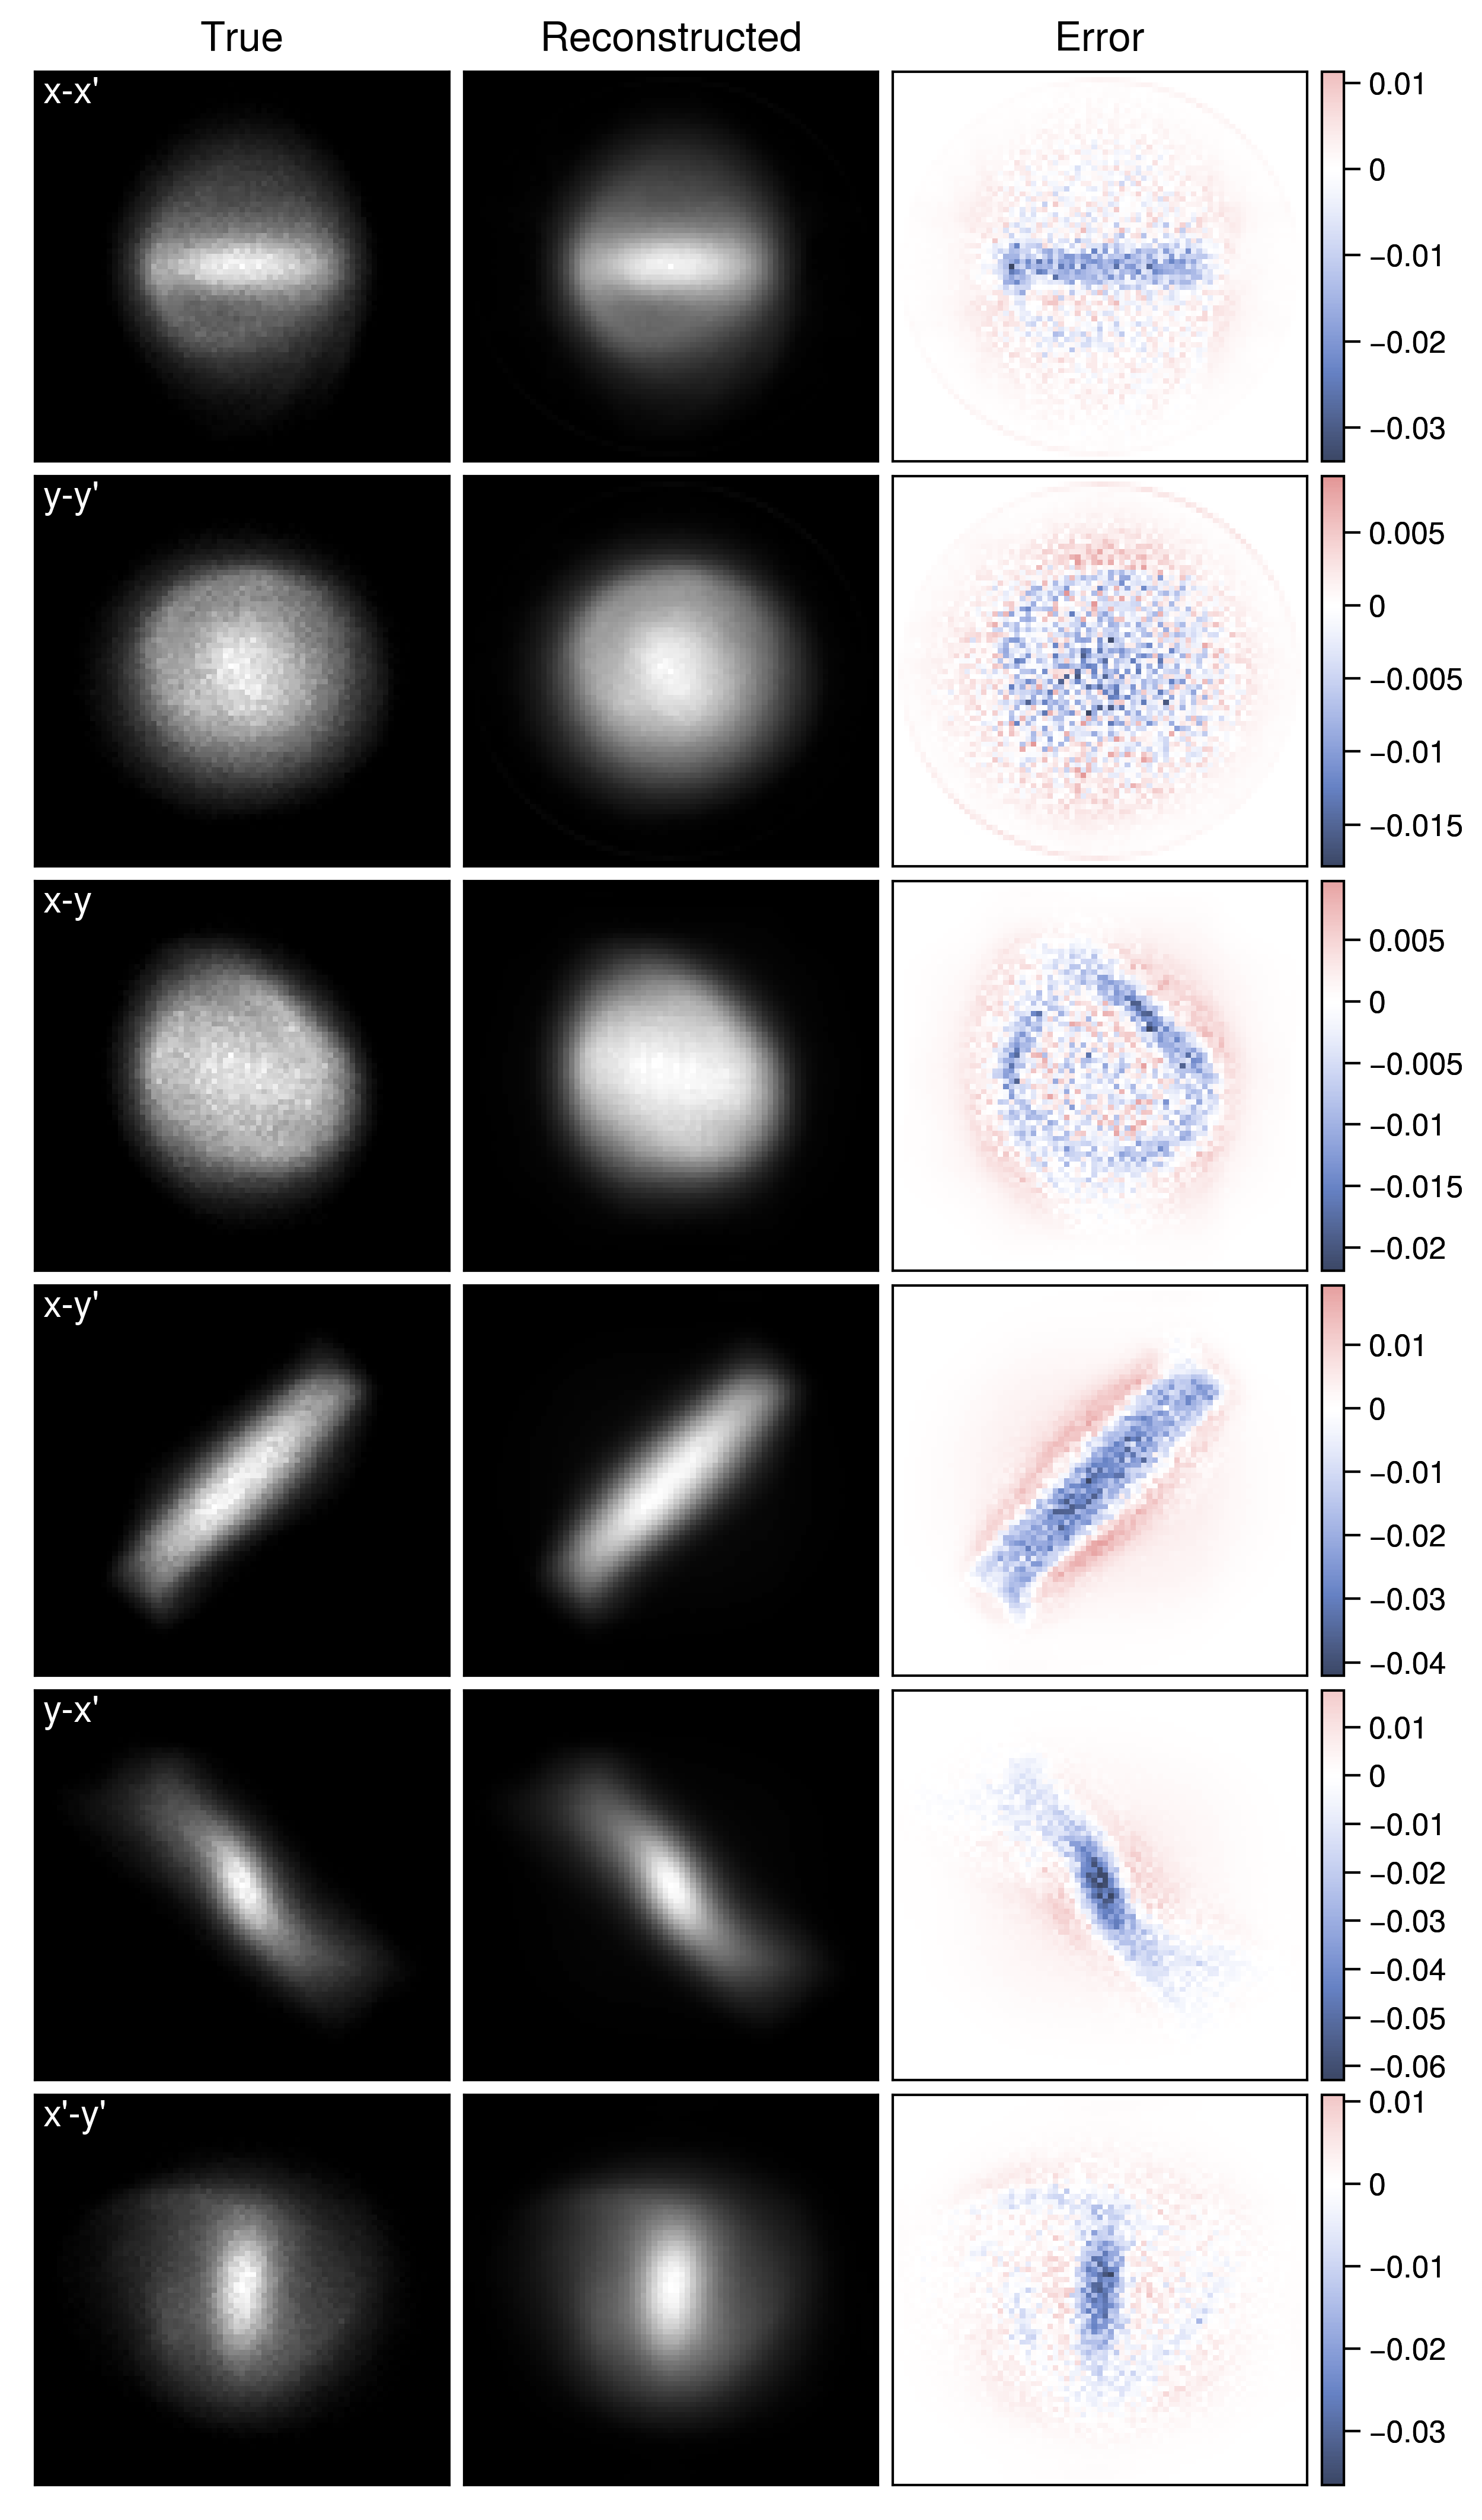
\includegraphics[width=0.8\textwidth]{Images/chapter4/tomo_sim_rec_hock_proj_2D_ver.png}
    \caption{Simulated reconstruction using Hock's method (normalized phase space).}
    \label{fig:tomo_sim_rec_hock_proj_2D}
\end{figure}
%
Notice that the projections of the reconstructed distribution, such as $x$-$y'$, are present in the simulated $x$-$y$ images in Fig.~\ref{fig:tomo_sim_target_scan}. The reason is straightforward: if the phase advance in the vertical plane is $\pi$/2, then $y \rightarrow y'$ and $f(x, y) \rightarrow f(x, y')$ \cite{Hock2013a}. 

This method is preferred because it leverages 2D reconstruction algorithms. Open-source implementations of these algorithms are widely available and the conditions needed for accurate reconstructions are well-understood, primarily due to the use of tomography in medical imaging.


\subsection{Direct 4D reconstruction}

If the phase advances cannot be independently controlled or if only a very small number of projections can be collected, 2D reconstruction algorithms must be generalized to 4D. Several algorithms generalize to any number of dimensions, but they may be difficult to implement, the conditions for an accurate reconstruction may be unclear, and the time and space complexity may make the method infeasible. Here, we focus on one method that has recently been experimentally demonstrated, then mention a few more that could be explored in future work.


\subsubsection{ART}

Each measured projection on the screen produces the following set of equations:
%
\begin{equation}\label{eq:art}
    \bm{\rho} = \mathbf{P} \bm{\psi}.
\end{equation}
%
$\bm{\rho}$ is a vector of the pixel intensities on the screen and $\bm{\psi}$ is a vector of the phase space coordinates on the reconstruction grid. To form $\mathbf{P}$, we place a particle at the center of each bin in the reconstruction grid and track the particles to the screen using the transfer matrix. $\mathbf{P}_{i, j} = 1$ if particle $j$ landed in bin $i$ on the screen; otherwise, $\mathbf{P}_{i, j} = 0$. The equations produced by subsequent measurements are stacked, and the resulting system of equations is solved using a sparse least squares solver. This method has been used to reconstruct the phase space distribution in the Compact Linear Accelerator for Research and Applications (CLARA), a low-energy test facility \cite{Wolski2020}.

For an $N \times N \times N \times N$ reconstruction grid, an $N \times N$ measurement grid, and $n$ measurements, $\bm{\rho}$ has $nN^2$ elements, $\bm{\psi}$ has $n N^4$ elements, and $\mathbf{P}$ has $n N^2 \times N^4$ elements. In practice, these significant storage requirements limit the resolution of the reconstruction grid to $N \approx 50$ \cite{Wolski2020}. In Fig.~\ref{fig:tomo_sim_rec_art_proj_2D}, the method was applied to the same simulated distribution, but $8 \times 8$ projections were used instead of $15 \times 15$.
%
\begin{figure}[!p]
    \centering
    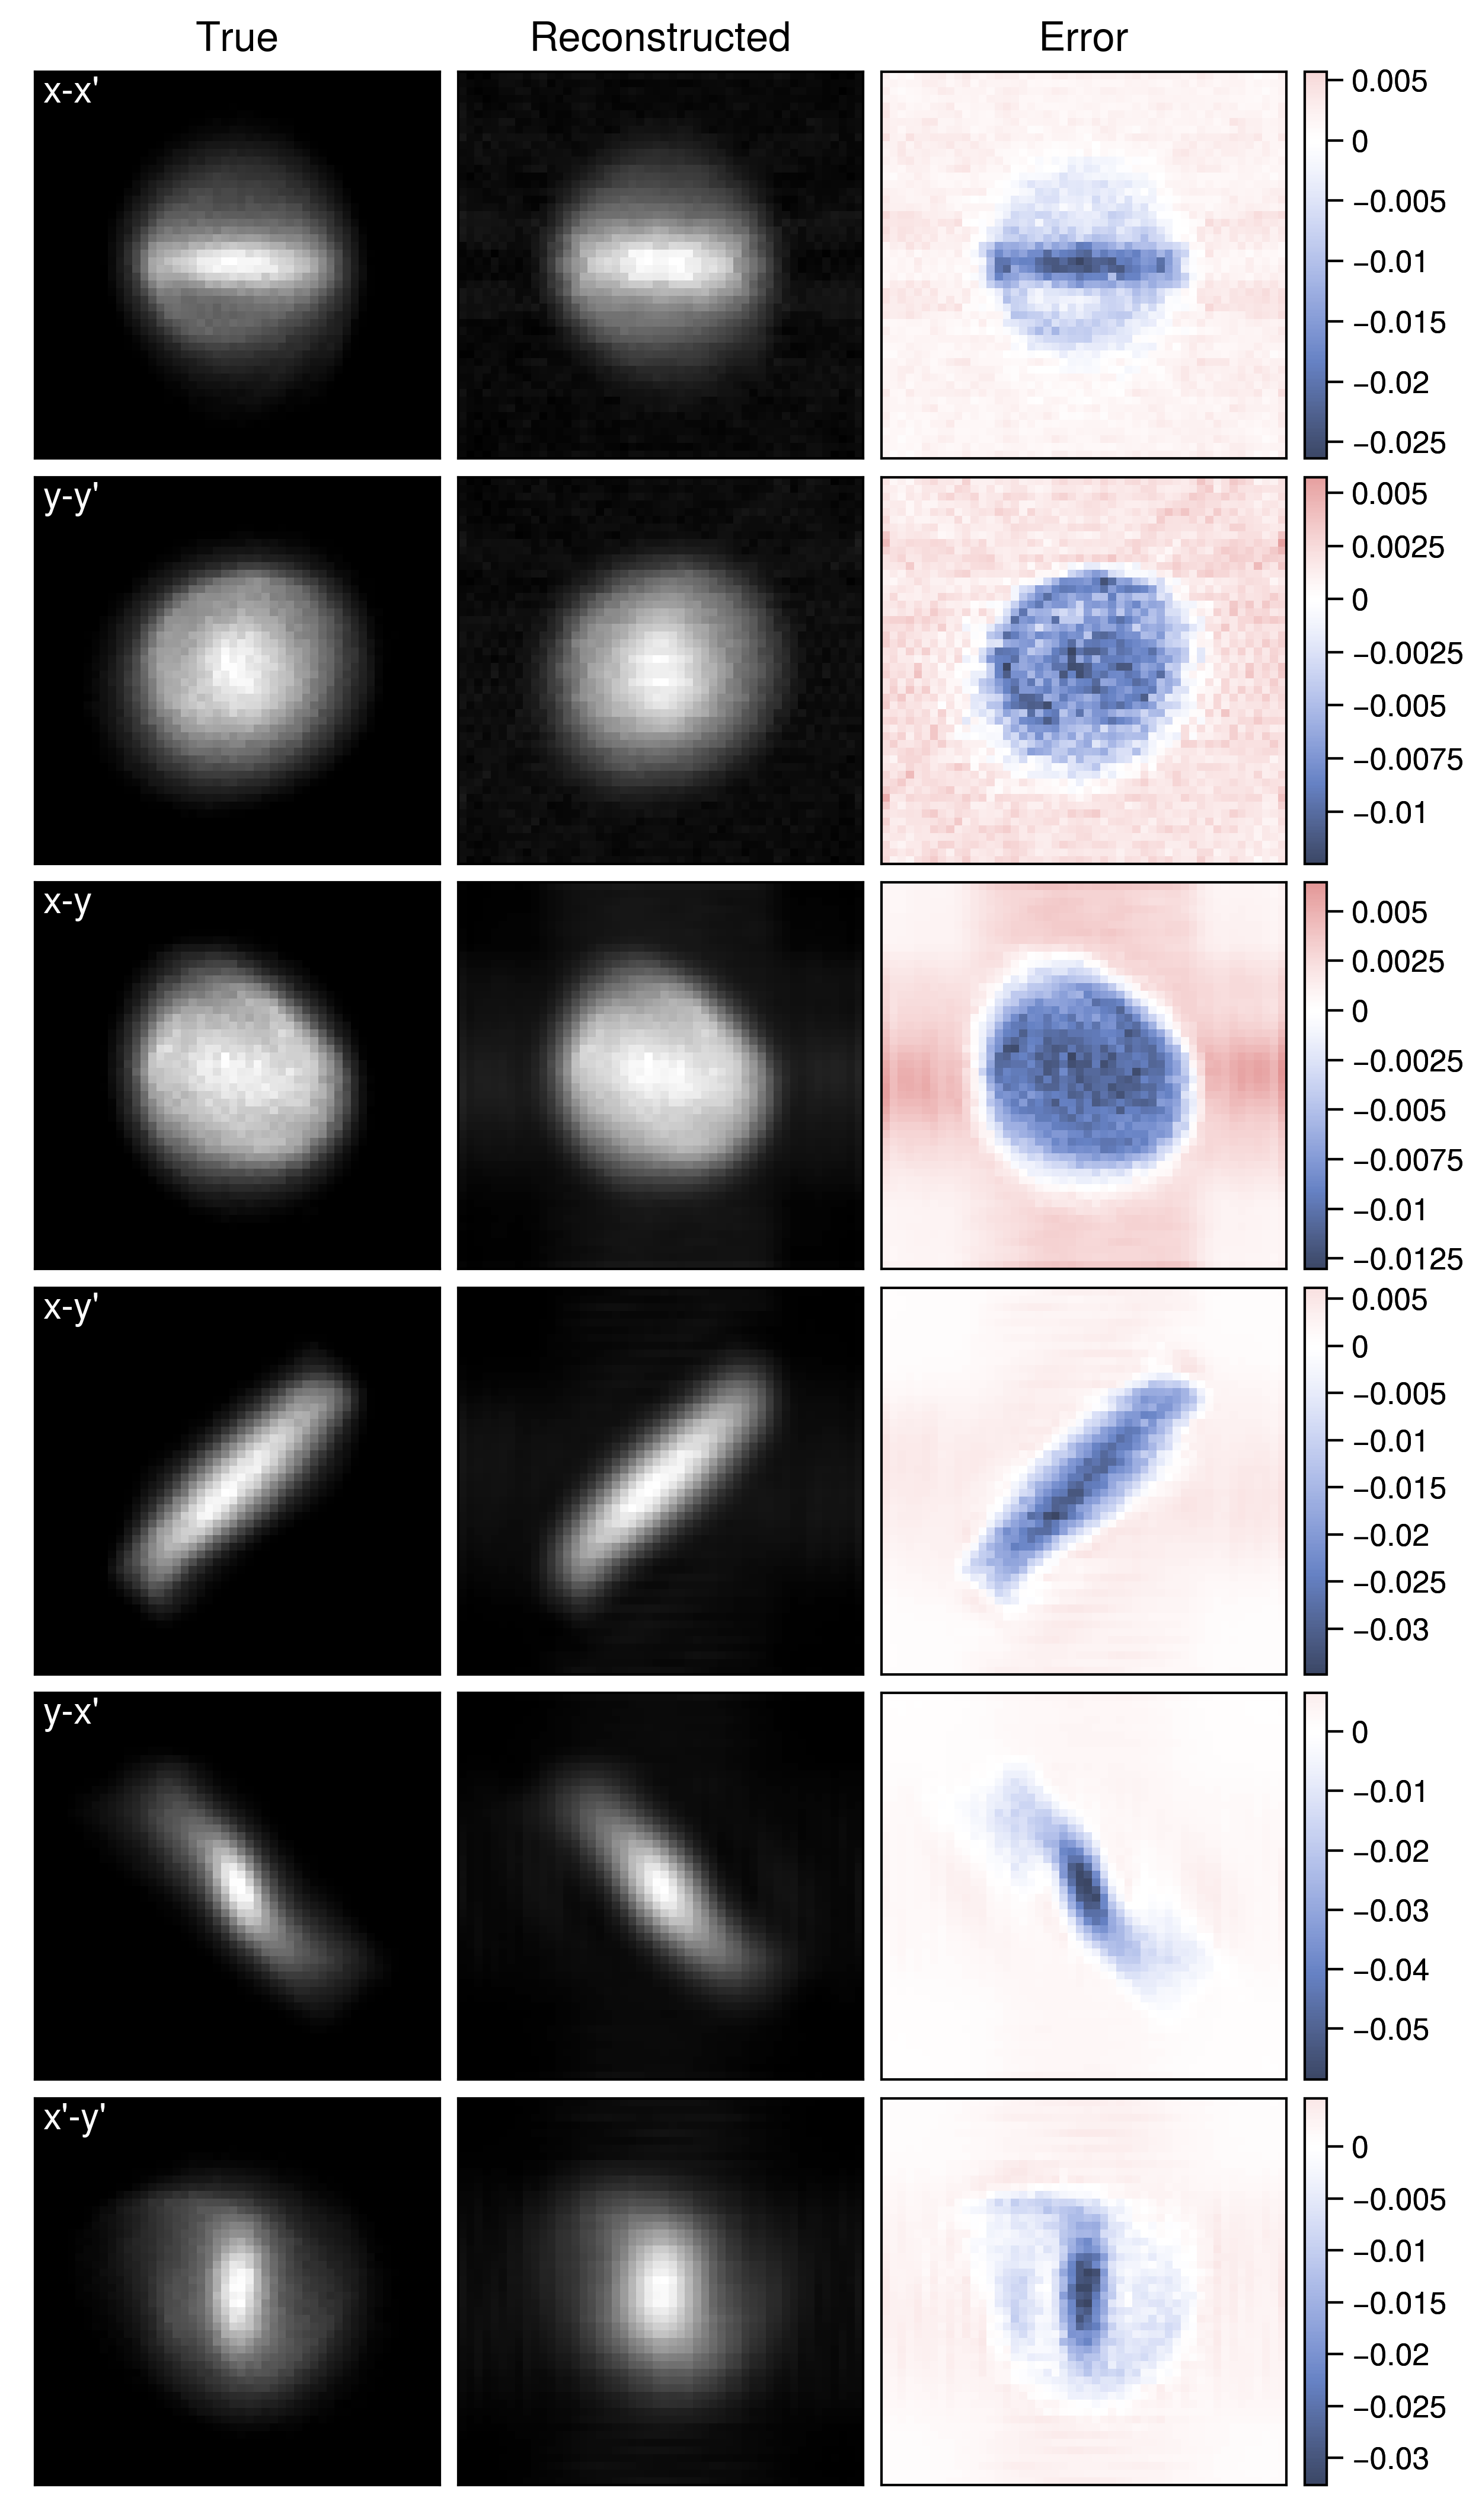
\includegraphics[width=0.8\textwidth]{Images/chapter4/tomo_sim_rec_art_proj_2D_ver.png}
    \caption{Simulated reconstruction using algebraic reconstruction (normalized phase space).}
    \label{fig:tomo_sim_rec_art_proj_2D}
\end{figure}
%
Although the main features of the distribution are present in the reconstruction, there are streaking artifacts outside the beam core that are not present in Fig.~\ref{fig:tomo_sim_rec_hock_proj_2D}, although is likely that the performance could improve if a larger number of projections were used. Unfortunately, the algorithm took hours to execute as opposed to minutes for the previous example, even with the reduced grid resolution.


\subsubsection{Additional methods}

Here are two additional methods to reconstruct the 4D phase space distribution that could be explored in future work.

Among the distributions consistent with the measured projections, MENT selects the distribution with the maximum entropy. For example, without any measurements constraining the solution, MENT will produce a uniform distribution. It can perform well with few projections and has been used for 2D reconstruction in particle accelerators \cite{Hock2013a}. The downside is that the iterative numerical solution is difficult to implement and may struggle to converge when the number of projections is large. For 4D reconstruction from $x$-$y$ projections, the MENT could be used to perform the 2D reconstructions in Hock's method, which may result in improved performance over SART. Alternatively, just as ART was generalized to four dimensions in the previous section, MENT could be generalized to four dimensions.\footnote{In principle, MENT can perform a 4D reconstruction using 1D projections \cite{Sander1979}; however, it seems a priori unlikely for this to produce an accurate result: imagine reconstructing a 3D image from 1D projections.} An analytic MENT solution has recently been derived and used for the 4D reconstruction of an SNS minipulse using $x$-$x'$ and $y$-$y'$ projections from a laser wire \cite{Wong-forthcoming}. 

Another method is to generate a particle bunch, track the bunch to the screen, weight each particle by the measured signal at the bin where it fell on the screen, and generate new particles in the region of that particle according to its weight. The advantage of this method is that it does not assume linear transport and that it can perform well with few projections. It was experimentally demonstrated by Wang et. al. in the Xi’an Proton Application Facility (XiPAF) using six projections \cite{Wang2019}. 



\subsection{Implementation in the SNS}

The idea to use SNS target images for tomographic reconstruction of the phase space distribution was proposed late in this research. Due to this fact, as well as time constraints and unexpected machine downtime, the methods described in the previous subsection were not able to be applied to real data; this is left for future work. Nonetheless, the following paragraphs describe how the reconstruction can be performed in the SNS.


\subsubsection{Optics control}

We desire independent control of the horizontal and vertical phase advances. The optics control developed for the wire-scanner measurement can be used here. The constraints are now that the $\beta$ functions remain below 30 m/rad in the wire-scanner region, below 100 m/rad before the target, and stay within 15\% of their nominal values at the target. Fig.~\ref{fig:target_phase_scan_1} shows that both the horizontal and vertical phase advances can be independently scanned in a 180$\degree$ range. Fig.~\ref{fig:target_phase_scan_2} overlays the $\beta$ functions and phase advances throughout the RTBT for every step in the scan, showing that the beam size constraints are not violated. The horizontal axis starts at the first varied quadrupole and ends at the target.
%
\begin{figure}[!p]
    \centering
    \vspace*{2.0cm}
    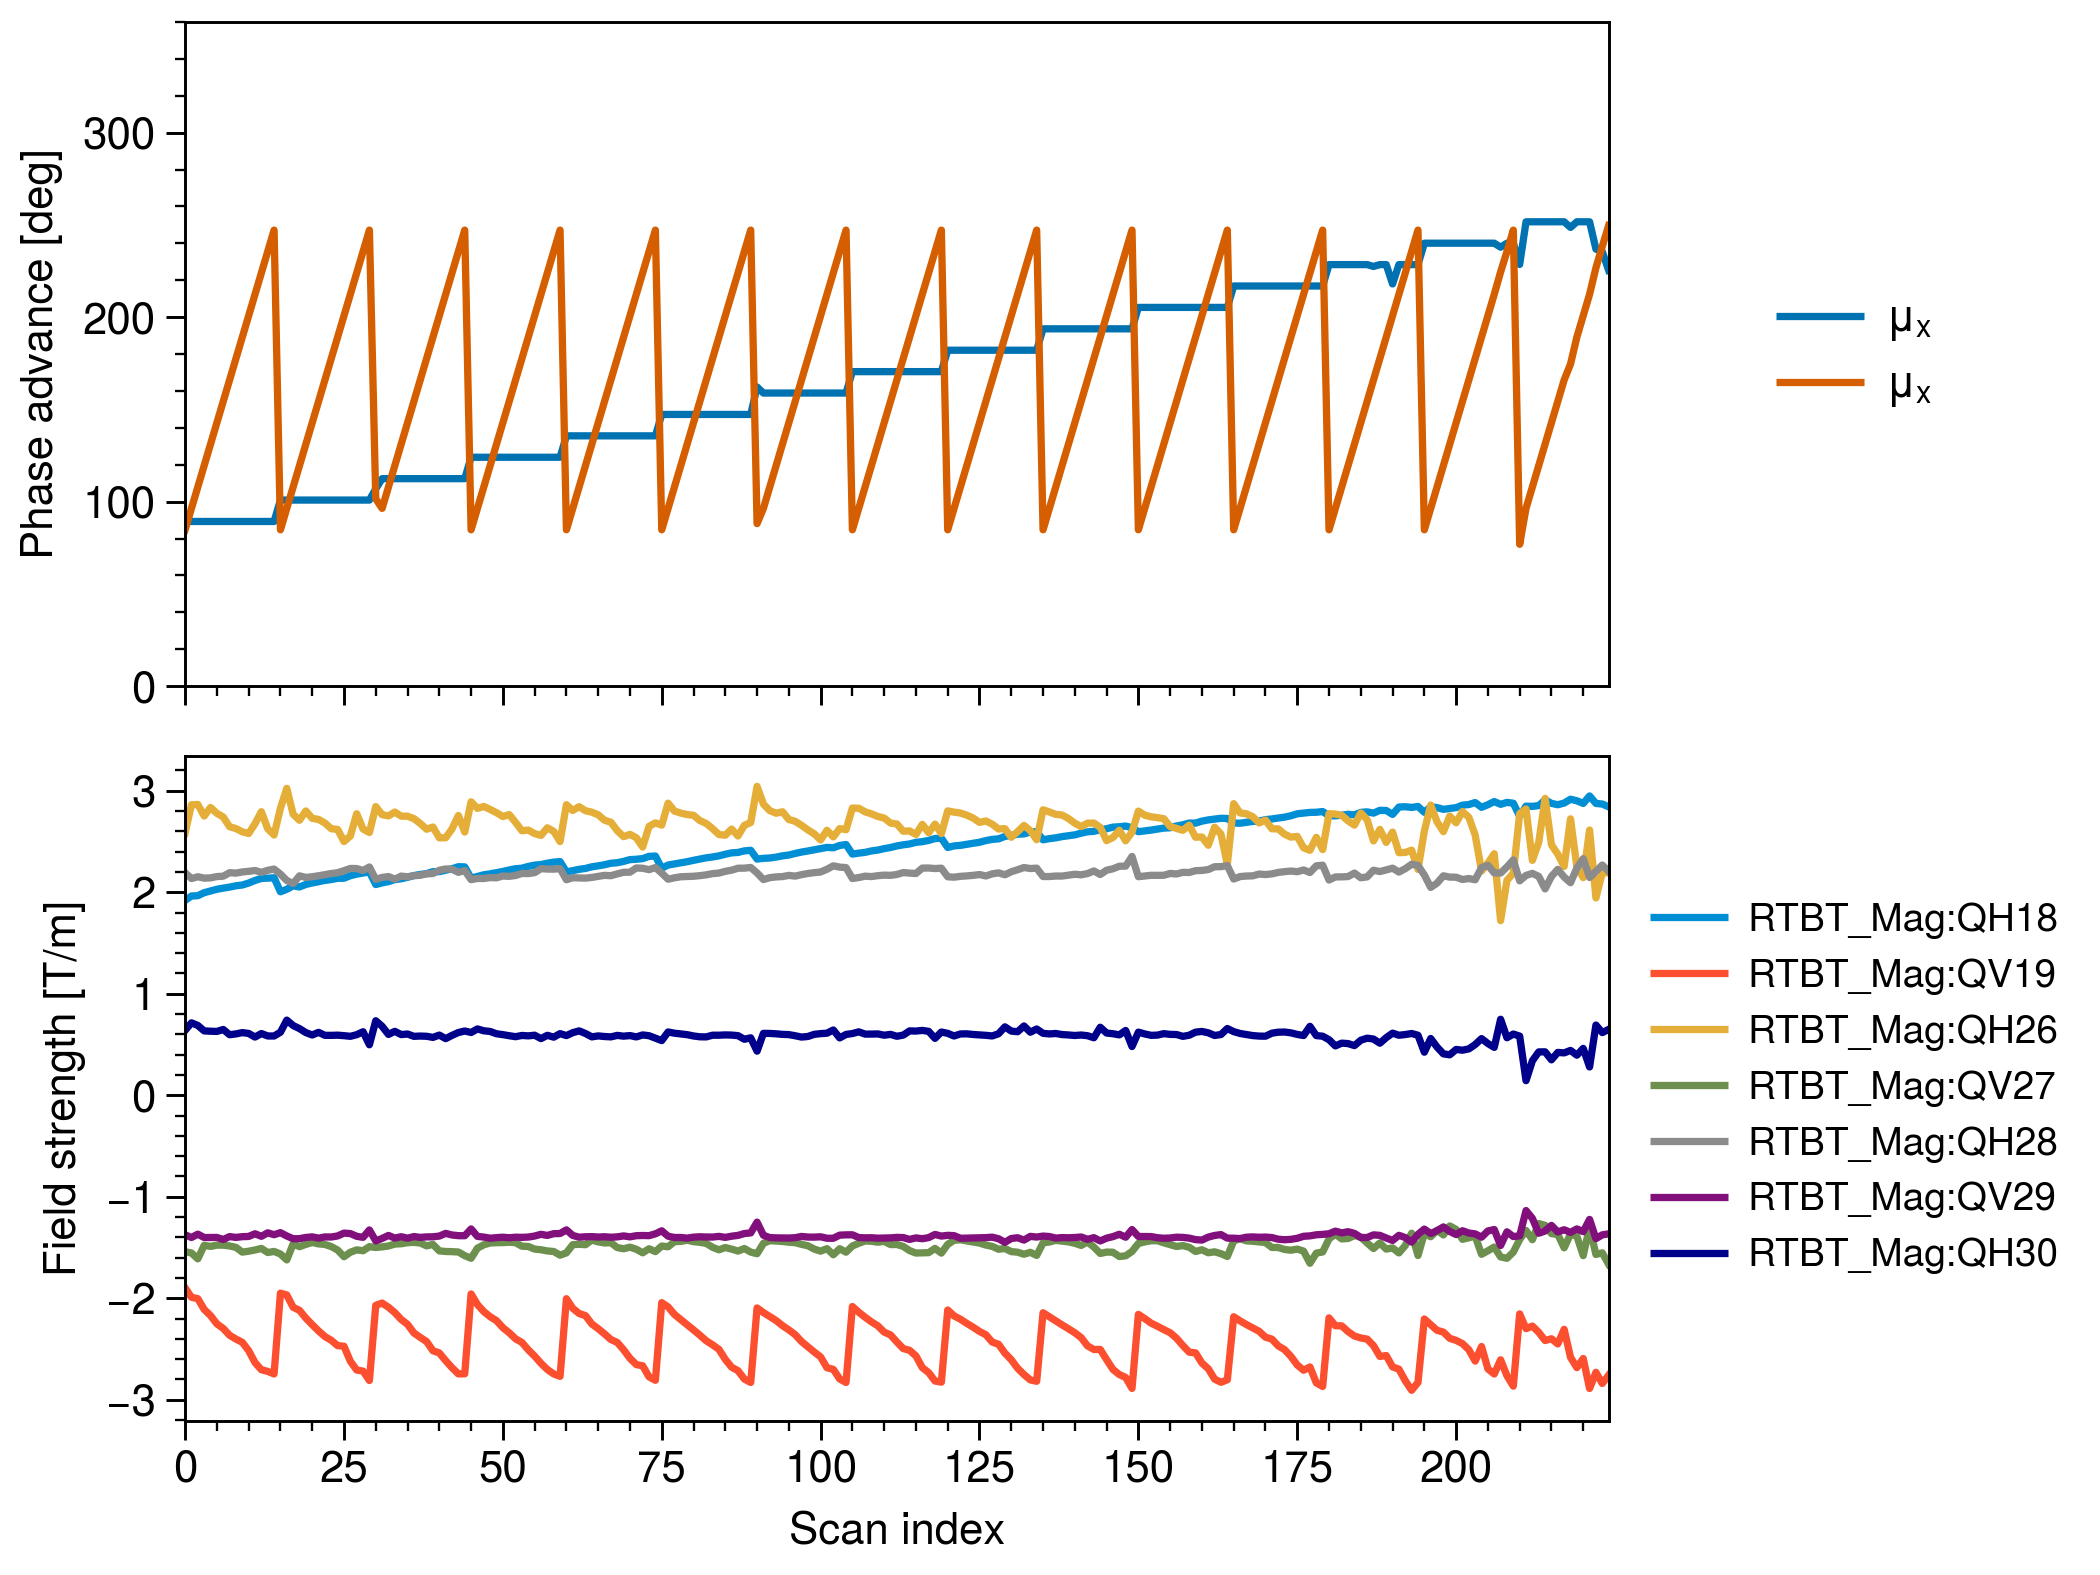
\includegraphics[width=\textwidth]{Images/chapter4/target_phase_scan1.png}
    \caption{Scan of the phase advances at the target.}
     \label{fig:target_phase_scan_1}
    \vspace*{2.0cm}
\end{figure}
%
\begin{figure}[!p]
    \centering
    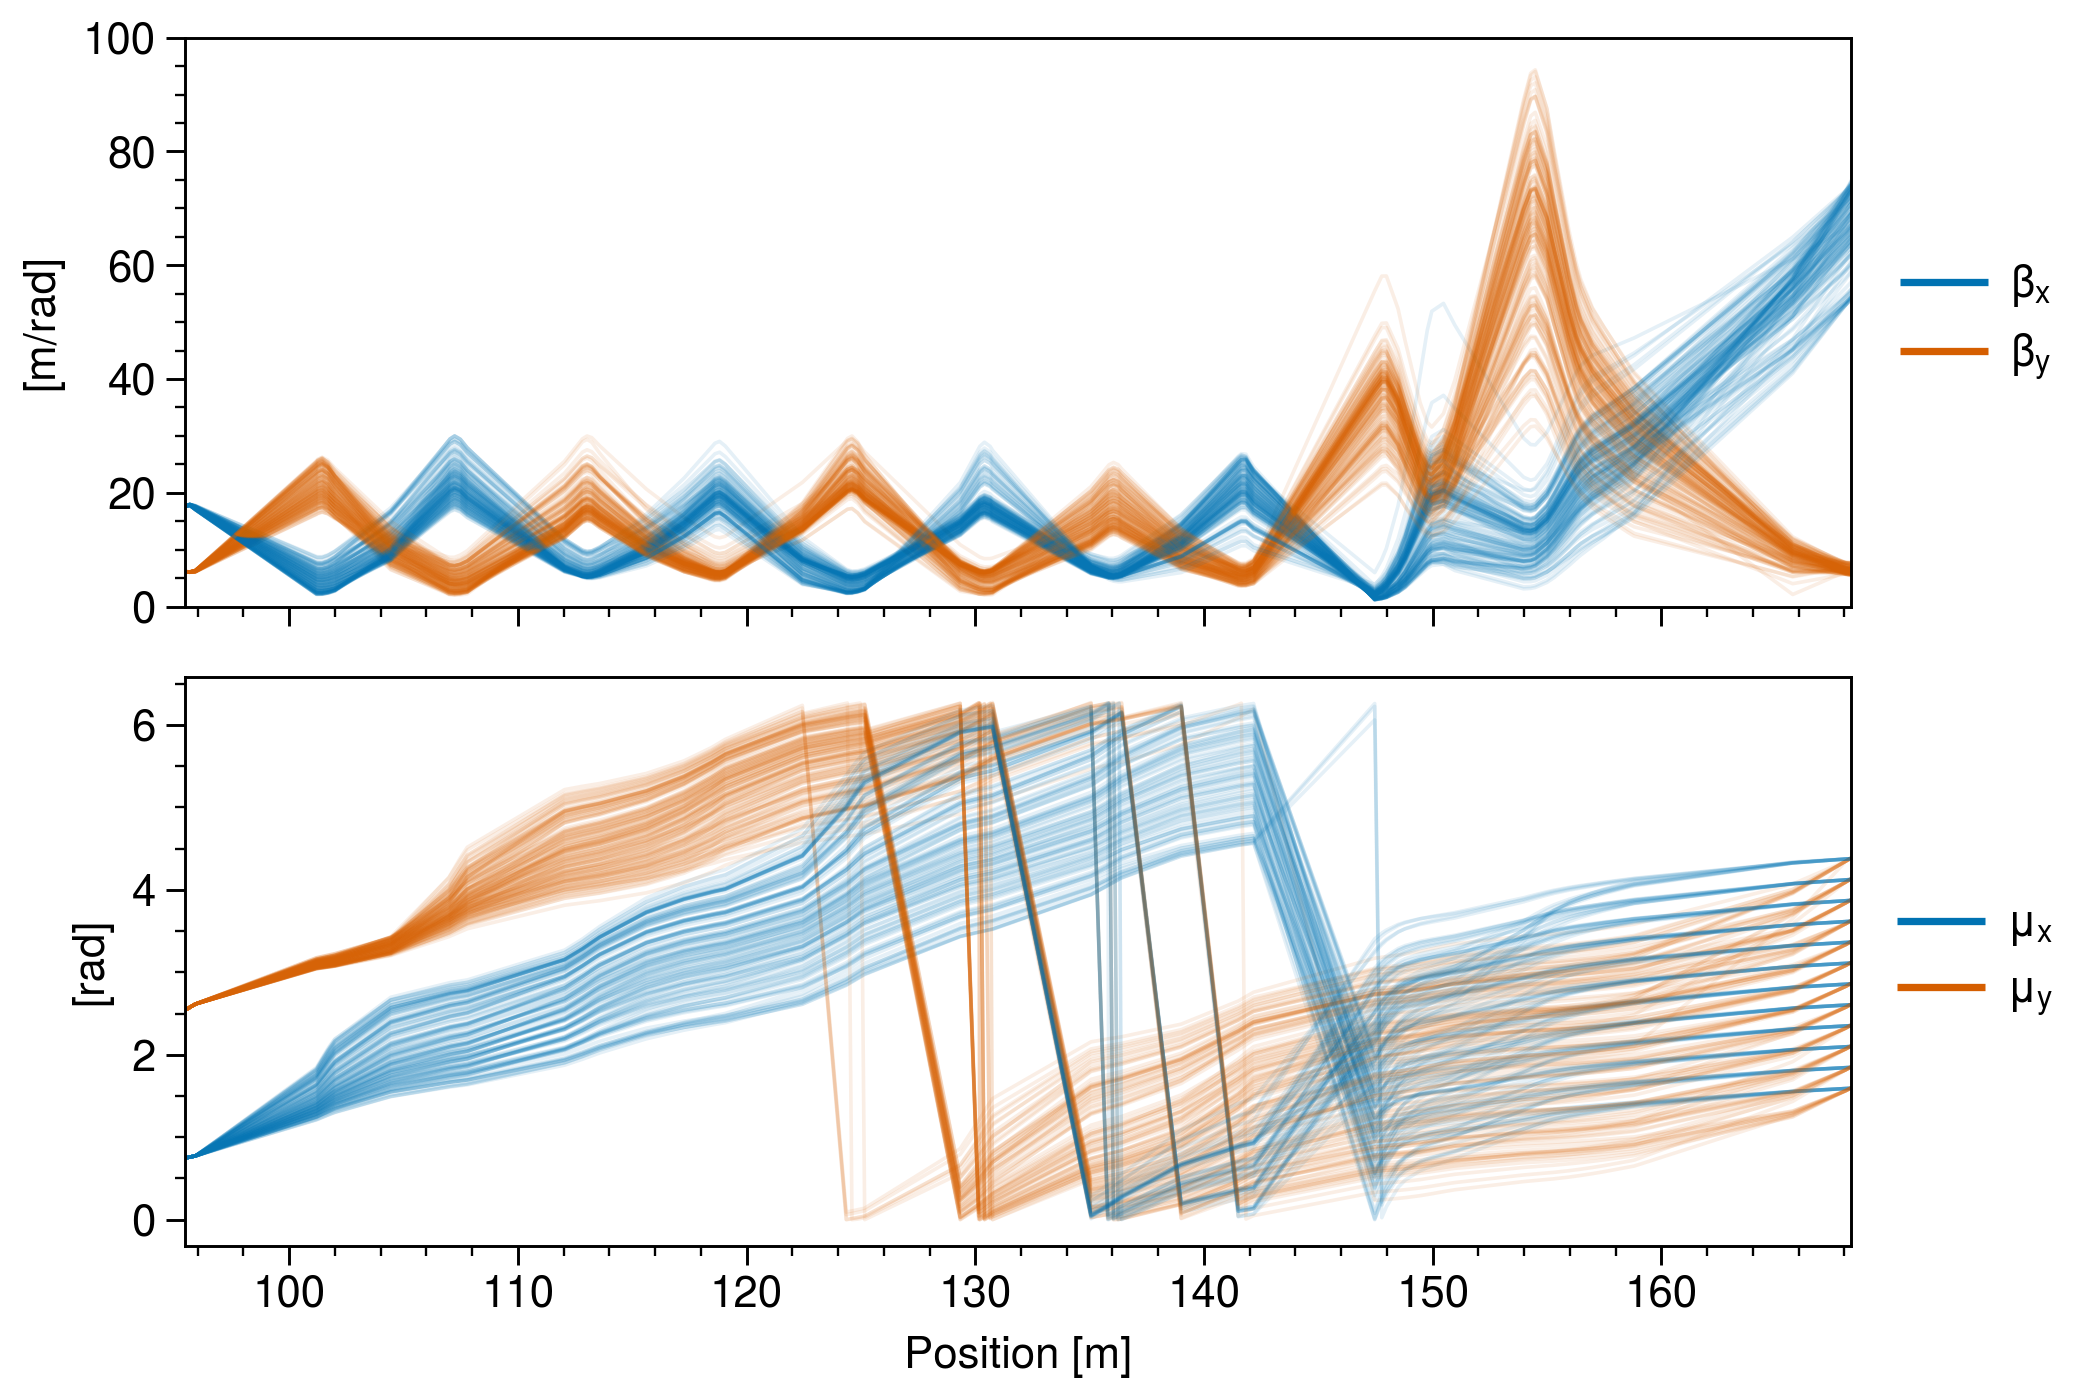
\includegraphics[width=\textwidth]{Images/chapter4/target_phase_scan2.png}
    \caption{$\beta$ functions and phase advances vs. position for the scan in Fig.~\ref{fig:target_phase_scan_1}.}
    \label{fig:target_phase_scan_2}
\end{figure}
%

Computing each optics setting takes approximately sixteen seconds using an OpenXAL solver. It also takes time to change the magnet strengths in the machine, trigger the beam, and collect a batch of target images. The time available in most accelerator physics studies is eight to ten hours at a maximum, so we place an upper limit on the number of images collected during the scan at $15 \times 15$, for which it takes around one hour to calculate the optics and one hour to collect the images. 


\subsubsection{Image acquisition and processing}

Target image acquisition is handled entirely by the target imaging system software. Live target images are displayed in the SNS control room. It is straightforward to access the image from an OpenXAL script as an 80,000 element array. The script to perform the target scan repeatedly modifies the RTBT quadrupoles, triggers the beam, and saves the image array to a file.

The unprocessed target images are not ideal. First, to reduce pulse-to-pulse variation, the images can be averaged over a few pulses. Second, the beam passes through 2 meters of Helium at atmospheric pressure before the target; due to radiation damage, light from the gas appears as a streaking artifact on the lower-right of the image \cite{Blokland2010}. Although this has been corrected by delaying the shutter opening by a few microseconds, the issue has occasionally resurfaced when the beam energy is different than 1 GeV. If these images are collected, they can be identified later by placing a maximum value on the pixels far from the image center, particularly in the lower-right region. Third, there are visible grid lines from the fiber bundle. A Gaussian blur is therefore applied to the image as in Fig.~\ref{fig:target_image}. Finally, there are four dark spots on the image that serve as fiducial markers; they are visible when the beam is large. In this work, the dark spots are left in the image.
%
\begin{figure}[!p]
    \centering
    \vspace*{5cm}
    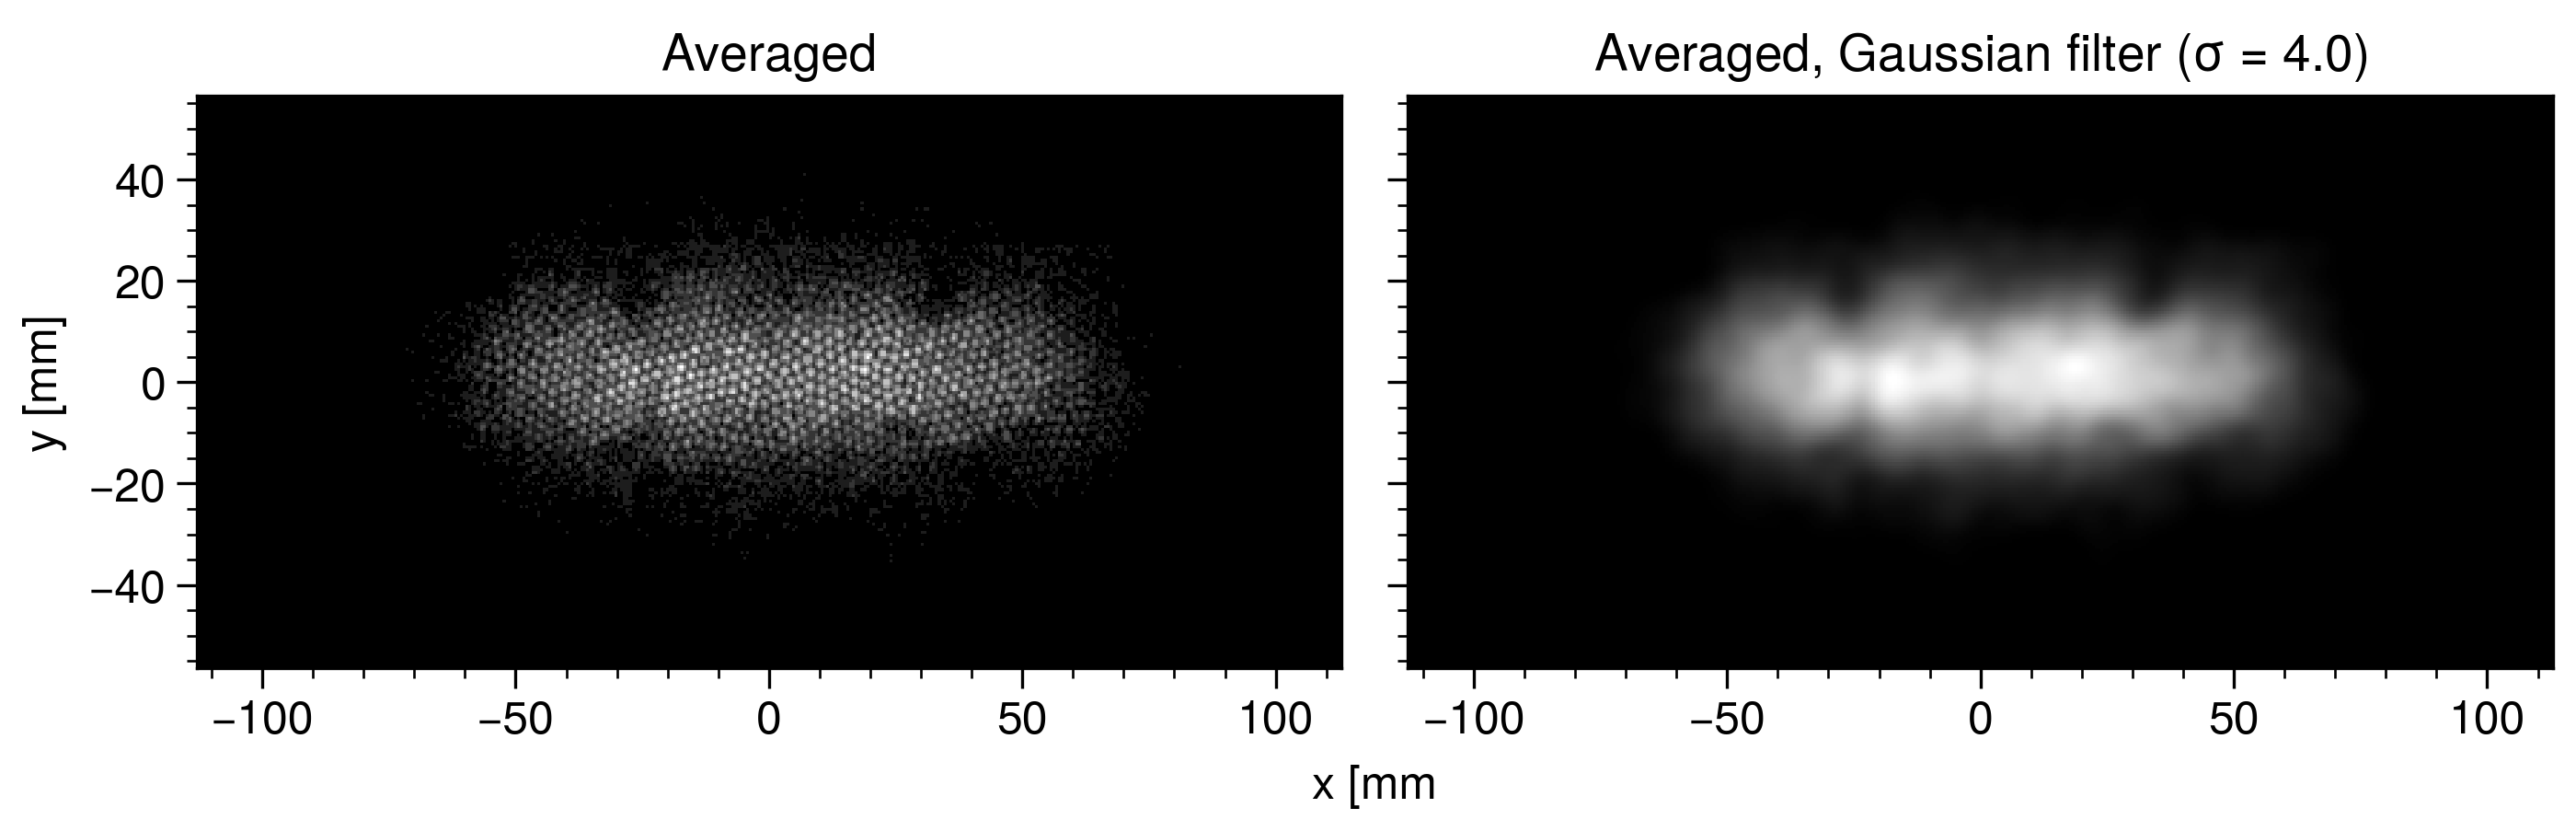
\includegraphics[width=1.0\textwidth]{Images/chapter4/target_image.png}
    \caption{Image of the beam on the target.}
    \label{fig:target_image}
     \vspace*{5cm}
\end{figure}
%


\subsubsection{Other uses of 2D projections}

There is information to be gained from 2D projections of the distribution in addition to the tomographic 4D reconstruction just described. The projections can be compared to a uniform density ellipse. Additionally, one can observe the variation in the $x$-$y$ correlation coefficient as the difference between the horizontal and vertical phase advances is varied. This reveals any ``hidden" cross-plane correlations, as in Fig.~\ref{fig:tomo_sim_target_scan}. Finally, by computing the RMS moments of the images, the covariance matrix can be reconstructed using the least squares method described in Section \ref{sec:Phase space reconstruction from 1D projections}; the advantage would be that data collection is much faster than for the wire-scanners and that the $\langle xy \rangle$ moment is computed directly.
